%% LyX 2.0.6 created this file.  For more info, see http://www.lyx.org/.
%% Do not edit unless you really know what you are doing.
\documentclass[11pt,english]{article}
\usepackage[T1]{fontenc}
\usepackage[latin9]{inputenc}
\usepackage{geometry}
\geometry{verbose,tmargin=3cm,bmargin=3cm,lmargin=3cm,rmargin=3cm,headheight=3cm,headsep=3cm,footskip=1.5cm}
\setlength{\parskip}{\bigskipamount}
\setlength{\parindent}{0pt}
\synctex=1
\usepackage{babel}
\usepackage{amsthm}
\usepackage{amsmath}
\usepackage{amssymb}
\usepackage{graphicx}
\usepackage{setspace}
\usepackage{esint}
\setstretch{1.5}
\usepackage[unicode=true,pdfusetitle,
 bookmarks=true,bookmarksnumbered=false,bookmarksopen=false,
 breaklinks=false,pdfborder={0 0 0},backref=false,colorlinks=false]
 {hyperref}

\makeatletter
%%%%%%%%%%%%%%%%%%%%%%%%%%%%%% Textclass specific LaTeX commands.
\numberwithin{equation}{section}
\theoremstyle{plain}
\newtheorem{thm}{\protect\theoremname}[section]
  \theoremstyle{plain}
  \newtheorem{cor}[thm]{\protect\corollaryname}
  \theoremstyle{plain}
  \newtheorem{lem}[thm]{\protect\lemmaname}
  \theoremstyle{plain}
  \newtheorem{prop}[thm]{\protect\propositionname}
  \theoremstyle{plain}
  \newtheorem{conjecture}[thm]{\protect\conjecturename}
  \theoremstyle{definition}
  \newtheorem{defn}[thm]{\protect\definitionname}
  \theoremstyle{definition}
  \newtheorem{example}[thm]{\protect\examplename}
  \theoremstyle{remark}
  \newtheorem{rem}[thm]{\protect\remarkname}
  \theoremstyle{remark}
  \newtheorem{claim}[thm]{\protect\claimname}

%%%%%%%%%%%%%%%%%%%%%%%%%%%%%% User specified LaTeX commands.
%bold caption labels
\usepackage[labelfont=bf]{caption}

\usepackage{ifthen}

%\allowdisplaybreaks

% clickable links
%\usepackage[bookmarks,hidelinks]{hyperref} 

%if I don't do this I get an error on URLs
\usepackage{url}

% list hackery
\usepackage{enumitem}
\setlist[enumerate]{label=\textup{(\roman*)},topsep=-5pt}
\setlist[itemize]{topsep=-5pt}

% cleveref allows \ref{thm:asdf} instead of Theorem~\ref{thm:asdf}
\usepackage[nameinlink,capitalise,noabbrev]{cleveref}
\AtBeginDocument{\renewcommand{\ref}[1]{\cref{#1}}}

% LyX won't let me include cleveref before theorem declarations so I need to redefine everything as a hack
\theoremstyle{plain}
\newtheorem{mythm}{\protect\theoremname}[section]
\renewenvironment{thm}{\begin{mythm}}{\end{mythm}}
\theoremstyle{definition}
\newtheorem{mydefn}[mythm]{\protect\definitionname}
\renewenvironment{defn}{\begin{mydefn}}{\end{mydefn}}
\theoremstyle{definition}
\newtheorem{myexample}[mythm]{\protect\examplename}
\renewenvironment{example}{\begin{myexample}}{\end{myexample}}
\theoremstyle{plain}
\newtheorem{myprop}[mythm]{\protect\propositionname}
\renewenvironment{prop}{\begin{myprop}}{\end{myprop}}
\theoremstyle{plain}
\newtheorem{mycor}[mythm]{\protect\corollaryname}
\renewenvironment{cor}{\begin{mycor}}{\end{mycor}}
\theoremstyle{plain}
\newtheorem{mylem}[mythm]{\protect\lemmaname}
\renewenvironment{lem}{\begin{mylem}}{\end{mylem}}
\theoremstyle{plain}
\newtheorem{myconjecture}[mythm]{\protect\conjecturename}
\renewenvironment{conjecture}{\begin{myconjecture}}{\end{myconjecture}}
\theoremstyle{remark}
\newtheorem{myrem}[mythm]{\protect\remarkname}
\renewenvironment{rem}{\begin{myrem}}{\end{myrem}}
\theoremstyle{remark}
\newtheorem{myclaim}[mythm]{\protect\claimname}
\renewenvironment{claim}{\begin{myclaim}}{\end{myclaim}}

% equation cref format
\crefformat{equation}{#2(#1)#3}

% make cref play nicely with different kinds of lists
\newlist{conditions}{enumerate}{3}
\setlist[conditions]{label=\textup{(\roman*)},topsep=-5pt}
\if@cref@capitalise
  \crefname{conditions}{Condition}{Conditions}
\else
  \crefname{conditions}{Condition}{Conditions}
\fi
\crefalias{conditionsi}{conditions}
\crefalias{conditionsii}{conditions}
\crefalias{conditionsiii}{conditions}

% ordered lists should use parens instead of a point
%\renewcommand\theenumi{\arabic{enumi}}
%\renewcommand\labelenumi{(\theenumi)}

% \left(\right) should behave the same as ()
\let\originalleft\left
\let\originalright\right
\renewcommand{\left}{\mathopen{}\mathclose\bgroup\originalleft}
\renewcommand{\right}{\aftergroup\egroup\originalright}

% table of contents spacing tweaks
\usepackage{tocloft}
\setlength\cftparskip{-2pt}
\setlength\cftbeforesecskip{1pt}
\setlength\cftaftertoctitleskip{2pt}

% comment environment
\usepackage{verbatim}

% mainly for light colours color!percent
\usepackage{xcolor}

% shaded WIP notes
\theoremstyle{definition}
\newtheorem{commentthm}{Comment}[section]
\newtheorem{todothm}[commentthm]{Issue}
\usepackage{framed}
\usepackage{lipsum}
\newenvironment{note}
{\colorlet{shadecolor}{blue!5}\begin{shaded}\begin{commentthm}}{\end{commentthm}\end{shaded}}
\newenvironment{todo}
{\colorlet{shadecolor}{red!5}\begin{shaded}\begin{todothm}}{\end{todothm}\end{shaded}}

%more distinct calligraphic letters
%\usepackage{calrsfs}

%theorem names in uppercase?
\let\oldtextbf\textbf
\renewcommand\textbf[1]{\uppercase{#1}}

%graph drawing
\usepackage{tikz}
\tikzstyle{vertex}=[circle,draw=black,fill=black,inner sep=0,minimum size=0.2cm,text=white,font=\footnotesize]
\tikzset{every loop/.style={min distance=50,in=50,out=130,looseness=7}}

\makeatother

  \providecommand{\claimname}{Claim}
  \providecommand{\conjecturename}{Conjecture}
  \providecommand{\corollaryname}{Corollary}
  \providecommand{\definitionname}{Definition}
  \providecommand{\examplename}{Example}
  \providecommand{\lemmaname}{Lemma}
  \providecommand{\propositionname}{Proposition}
  \providecommand{\remarkname}{Remark}
\providecommand{\theoremname}{Theorem}

\begin{document}
\begin{titlepage}


\title{
\includegraphics[scale=0.3]{crest_4}\vfill{}
Stein's Method}


\author{Matthew Kwan\\
Supervisor: Catherine Greenhill\\
\\
School of Mathematics,\\
The University of New South Wales}

\maketitle
\noindent \begin{center}
\vfill{}
Submitted in partial fulfillment of the requirements of the degree
of\\
Bachelor of Science with Honours
\par\end{center}

\thispagestyle{empty}\end{titlepage}

\begin{comment}
\begin{thm}
t\end{thm}
\begin{cor}
c\end{cor}
\begin{lem}
l\end{lem}
\begin{prop}
p\end{prop}
\begin{conjecture}
c\end{conjecture}
\begin{defn}
d\end{defn}
\begin{example}
e\end{example}
\begin{rem}
r\end{rem}
\begin{claim}
c
\end{claim}
\end{comment}

\global\long\def\floor#1{\left\lfloor #1\right\rfloor }


\global\long\def\ceil#1{\left\lceil #1\right\rceil }


\global\long\def\i{i}


\global\long\def\ii{j}


\global\long\def\iii{q}


\global\long\def\iiii{r}


\global\long\def\NN{\mathbb{N}}


\global\long\def\ZZ{\mathbb{Z}}


\global\long\def\RR{\mathbb{R}}


\global\long\def\CC{\mathbb{C}}


\global\long\def\F{\mathcal{F}}


\global\long\def\range#1{\left[#1\right]}


\global\long\def\rest{|}


\global\long\def\d{\operatorname d}


\global\long\def\id{\operatorname{id}}


\global\long\def\one{\operatorname{\boldsymbol{1}}}


\global\long\def\falling#1#2{\left(#1\right)_{#2}}


\tableofcontents{}

\begin{todo}Remaining stuff:
\begin{itemize}
\item random combinatorial structures: merge?
\item size-bias coupling
\item finish proof sketch for random regular graphs section
\item further reading
\end{itemize}
\end{todo}


\section{Introduction}

The \emph{\textbf{c}entral \textbf{l}imit \textbf{t}heorem}, roughly
speaking, says that sums of independent, identically distributed random
variables are ``approximately normal'', with the approximation improving
as the number of terms in the sum increases. Similarly, the \emph{Poisson
\textbf{l}imit \textbf{t}heorem} says that the number of occurences
of independent ``rare'' events over a given time period is ``approximately
Poisson''. These two limit theorems are archetypal examples of a
large class of related results in statistics and probabilistic combinatorics.

These types of results are generally formally stated asymptotically,
with a particular type of convergence called \emph{weak convergence},
or \emph{convergence in distribution}. Such results are very powerful,
but an obvious shortcoming is that they do not ``quantify'' the
convergence. It may be that a sequence of random variables is ``asymptotically
normal'', but we cannot say that any particular random variable in
that sequence is individually ``close to normal''. Even if we are
only interested in asymptotic results, it can be problematic that
we cannot say convergence is ``uniform'' in any sense.

The solution to both these problems is to define a distance metric
between probability distributions, and study convergence with respect
to this metric. Fortunately, weak convergence is in fact convergence
with respect to a topology, and this topology is metrizable. That
is, there is a metric on the set of probability distributions such
that convergence in this metric space is equivalent to weak convergence.

\emph{Stein's method }was introduced by Charles Stein in 1972. It
is most generally a method for approximating expected values. However,
at least in probabilistic combinatorics, Stein's method has proved
especially useful for bounding the distance between probability distributions,
in a variety of metrics consistent with weak convergence. Such bounds
can be used to quantify existing limit theorems, and can also be used
as a tool to prove purely asymptotic results.

In this thesis, we set out the theoretical groundwork for Stein's
method, including an overview of basic probability theory and a discussion
of weak convergence. We then present a very general framework for
the Stein's method, and outline a few particular ways of applying
the method. We include a number of specific examples and applications.

Unless stated otherwise, all proofs are ``original'' in that I came
up with them, although many are quite straightforward and probably
exist elsewhere. For the proofs that I have adapted from other sources
(which are all cited), I tried to add value with clearer explanation
and filling in skipped steps, or by adapting (and simplifying) the
proof for a special case.


\subsection{Notation and Assumed Knowledge}

For this thesis, the set of natural numbers $\NN$ includes zero.
We write $\one_{A}$ for the characteristic function of a set $A$;
that is, $\one_{A}\left(x\right)=1$ if $x\in A$, otherwise $\one_{A}\left(x\right)=0$.
The function $f$ restricted to the set $A$ is denoted $f\rest_{A}$.
The falling factorial $n\left(n-1\right)\dots\left(n-k+1\right)$
is denoted $\falling nk$. Finally, $\range k$ denotes the set $\left\{ 1,\dots,k\right\} $. 

Unless otherwise specified, all asympotics are as $n\to\infty$. Apart
from standard asymptotic notation, $f\sim g$ means $f=g\left(1+o\left(1\right)\right)$.

\begin{comment}, $f\prec g$ means $f=O\left(g\right)$ and $f\asymp g$
means $f=\Theta\left(g\right)$.\end{comment}

I will occasionally use results from analysis without proof. I will
usually refer to a numbered theorem in Rudin's \emph{Real and Complex
Analysis} \cite{Rud66} or \emph{Functional Analysis} \cite{Rud73}
when doing so.

I will also assume some familiarity with basic graph theory definitions
and terminology. The reader may refer to a textbook such as \cite{Die00}
if necessary. We also specify some conventions here. Unless stated
otherwise, graphs are labelled. That is, they are distinguished even
within isomorphism classes. A graph may not have loops or multiple
edges; an object which is allowed to have loops and/or multiple edges
will be called a multigraph. See \ref{fig:graph-conventions}. We
write $G\subseteq G'$ to indicate that $G$ is a (not necessarily
induced) subgraph of $G'$.

\begin{figure}[h]
\begin{center}
\foreach \j in {1,2,3}
{
\hspace{0.5cm}
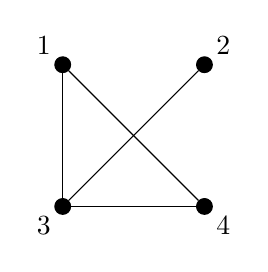
\begin{tikzpicture}[scale=.6]
\node[vertex] (1) at (0,3) {};
\node at (-0.4,3.4) {\ifthenelse{\equal{\j}{3}}{2}{1}};
\node[vertex] (4) at (3,0) {};
\node at (3.4,-0.4) {4};
\node[vertex] (3) at (0,0) {};
\node at (-0.4,-0.4) {3};
\node[vertex] (2) at (3,3) {};
\node at (3.4,3.4) {\ifthenelse{\equal{\j}{3}}{1}{2}};
\ifthenelse{\equal{\j}{1}}{
\path
(1) edge [bend right] (3)
    edge [bend left] (3)
    edge (2)
(4) edge (3)
    edge [loop right,-] (4)
(2) edge (3);
}
{
\path
(1) edge (3)
    edge (4)
(4) edge (3)
(2) edge (3);
}
\end{tikzpicture}
\hspace{0.5cm}
}
\end{center}

\caption{\label{fig:graph-conventions}From left to right: a multigraph that
is not a graph, and two different graphs on the vertex set $\left\{ 1,2,3,4\right\} $.}
\end{figure}



\section{General Probability Theory}

\global\long\def\L#1{\mathcal{L}_{#1}}


\DeclareRobustCommand{\L}[1]{\ifmmode{\mathcal{L}_{#1}}\else\polishL\fi}

\global\long\def\Lb#1{\mathcal{L}\left(#1\right)}


\global\long\def\Om{\Omega}


\global\long\def\om{\omega}


\global\long\def\cA{\mathcal{A}}


\global\long\def\B{\mathcal{B}}


\global\long\def\E{\mathbb{E}}


\global\long\def\F{F}


\global\long\def\N{\mathcal{N}}


\global\long\def\Po{\operatorname{Po}}


\global\long\def\Var{\operatorname{Var}}


\global\long\def\im{\operatorname{im}}


\global\long\def\sgn{\operatorname{sign}}


\global\long\def\supp{\operatorname{supp}}


\global\long\def\Pr{\mathbb{P}}


\global\long\def\m{\mu}


\global\long\def\X{X}


\global\long\def\bX{\mathbf{X}}


\global\long\def\A{A}


\global\long\def\P{\mathcal{P}}


For many combinatorial applications, an informal understanding of
probability theory (often considering only discrete spaces) will suffice.
However, in this thesis a rigorous foundation in probability theory
will be useful. This section will therefore assume knowledge of basic
measure theory; see, for example, \cite{Rud66}. However, where possible,
we will note any simplifications that arise from assuming discreteness.

No knowledge of probability theory is assumed; the first few subsections
will briefly review the foundations of probability. The reader may
nevertheless want to refer to a probability theory book such as \cite{Kal02}
for some additional detail and further reading.


\subsection{Probability Spaces}
\begin{defn}
A \emph{probability space} is a measure space $\left(\Om,\cA,\Pr\right)$
with $\Pr\left(\Om\right)=1$. In this case we say $\Pr$ is a \emph{probability
measure}, and denote the set of all probability measures on $\left(\Om,\cA\right)$
by $\P\left(\Om,\cA\right)$ or $\P\left(\Om\right)$ if there is
no ambiguity.\end{defn}
\begin{rem}
\label{rem:discrete-space}For our purposes $\Om$ will often be countable,
with $\cA$ as the power set of $\Om$. In this case $\Pr$ is uniquely
defined by the probabilities $\Pr\left(\om\right):=\Pr\left(\left\{ \om\right\} \right)$,
for each $\om\in\Om$. We will discuss specific probability spaces
on sets of combinatorial objects in \ref{sec:random-structures}.\end{rem}
\begin{defn}
An \emph{event} in a probability space $\left(\Om,\cA,\Pr\right)$
is a measurable set $\A\in\cA$.
\end{defn}
For an event $\A$, $\Pr\left(\A\right)$ is interpreted as the ``probability
that $\A$ occurs''. Events will usually be of the form $\A=\left\{ \om\in\Om:\, P\left(\om\right)\mbox{ holds}\right\} $,
where $P\left(\om\right)$ is some property of an object $\om$. For
clarity, we often abuse notation slightly and write $\Pr\left(P\mbox{ holds}\right)$
instead of $\Pr\left(\left\{ \om\in\Om:\, P\left(\om\right)\mbox{ holds}\right\} \right)$.


\subsection{Random Elements}
\begin{defn}
A \emph{random element} is a measurable function $\X:\left(\Om_{1},\cA_{1}\right)\to\left(\Om_{2},\cA_{2}\right)$
between measurable spaces. If $\Om_{2}=\RR^{n}$ for some $n\in\NN$,
with $\cA_{2}$ the Borel $\sigma$-algebra on $\RR^{n}$, then we
say $\X$ is a \emph{random vector}. A one-dimensional random vector
is a \emph{random variable}. If $\Om_{2}$ is countable then we say
$\X$ is \emph{discrete}.\end{defn}
\begin{rem}
Especially in combinatorial spaces, $\Om_{1}$ is often countable.
In this case, any function from a probability space $\left(\Om_{1},2^{\Om_{1}},\Pr\right)$
is measurable.
\end{rem}
To interpret a random variable, we need a probability measure $\Pr$
on the underlying measurable space $\left(\Om_{1},\cA_{1}\right)$
(often, this will be implicit). Then, $\Pr\left(\X\in\A\right)=\Pr\left(\left\{ \om\in\Om_{1}:\X\left(\om\right)\in\A\right\} \right)$
is the probability that $\X$ takes a value in the set $\A$. Often,
we will only be interested in such probabilities: that is, we do not
care about the realization of a random variable as a function on an
underlying probability space. This motivates the following definition:
\begin{defn}
Suppose $\X$ is a random element which takes values in the measurable
space $\left(\Om,\cA\right)$. The \emph{distribution} (or \emph{law})
$\L{\X}$ of $\X$ with respect to an underlying probability $\Pr$
is the pushforward measure with respect to $\X$. That is, it is a
probability measure defined by $\L{\X}\left(\A\right)=\Pr\left(\X^{-1}\left(\A\right)\right)$
for $\A\subseteq\cA$. Also, we occasionally use the notation $\Lb{\X}:=\L{\X}$
for ease of reading.
\end{defn}
It is worth noting that in fact any probability measure is the distribution
of some random element, so we can define a probability distribution
abstractly and then assert the existence of a random variable with
that distribution. To see this, note that given a probability measure
$\L{}\in\P\left(\Om\right)$, we can choose $\X=\id_{\Om}$ to have
$\L{\X}=\L{}$ with respect to the underlying probability measure
$\L{}$. We also use the notation $\X\in\L{}$ to indicate that $\X$
has distribution $\L{}$.
\begin{example}
The normal distribution with parameters $\mu$ and $\sigma$ is denoted
$\N\left(\mu,\sigma\right)$ or $\N_{\mu,\sigma}$ and is defined
by 
\[
\N_{\mu,\sigma}\left(B\right)=\frac{1}{\sigma\sqrt{2\pi}}\int_{B}e^{-\frac{\left(x-\mu\right)^{2}}{2\sigma^{2}}}\d x
\]
 for any Borel set $B$.
\end{example}

\begin{example}
The Poisson distribution with parameter $\lambda$ is denoted $\Po\left(\lambda\right)=\Po_{\lambda}$;
this is defined by 
\[
\Po_{\lambda}\left(k\right)=\frac{\lambda^{k}e^{-\lambda}}{k!}
\]
 for all $k\in\NN$ (see \ref{rem:discrete-space}).
\end{example}
It is in general a little tricky to define ``the set of values a
random element can take'', but this is straightforward in the discrete
case.
\begin{defn}
The \emph{support} of a discrete random element $\X$ is the set 
\[
\supp\left(\X\right)=\left\{ k\in\Om:\Pr\left(\X=k\right)>0\right\} .
\]

\end{defn}

\subsection{Dependence and Coupling}
\begin{defn}
Suppose $\X$ and $\X'$ are random elements $\left(\Om_{1},\cA_{1},\Pr\right)\to\left(\Om_{2},\cA_{2}\right)$.
We say that $\X$ and $\X'$ are \emph{independent} if 
\[
\Pr\left(\X\in\A_{2}\right)\Pr\left(\X'\in\A_{2}\right)=\Pr\left(\X\in\A_{2}\mbox{ and }\X'\in\A_{2}\right)
\]
for all $\A_{2}\in\cA_{2}$. If $\A_{1},\A_{1}'\in\cA$ then we analogously
say $\A_{1}$ and $\A_{1}'$ are independent if 
\[
\Pr\left(\A_{1}\right)\Pr\left(\A_{1}'\right)=\Pr\left(\A_{1}\cap\A_{1}'\right).
\]
We can similarly say an event is independent of a random element.
If two objects are not independent, then we say they are \emph{dependent}.
\end{defn}
Intuitively, two objects are dependent if information about one object
can give information about the other. For example, we might be interested
in the probability of an event $\A$, under the assumption that the
event $\A'$ occurs.
\begin{defn}
The \emph{conditional probability} of an event $\A$, given an event
$\A'$ which has nonzero probability, is $\Pr\left(\A|\A'\right)=\Pr\left(\A\cap\A'\right)/\Pr\left(\A'\right)$.
\end{defn}
We have $\Pr\left(\A|\A'\right)=\Pr\left(\A\right)$ if and only if
$\A$ and $\A'$ are independent.

We can also condition random elements on an event.
\begin{defn}
Suppose $\X:\left(\Om_{1},\cA_{1},\Pr\right)\to\left(\Om_{2},\cA_{2}\right)$
is a random element, and $\A_{1}\in\cA_{1}$ is an event with nonzero
probability. Then the \emph{distribution of $\X$ conditioned on $\A_{1}$}
is denoted by $\L{\X|\A_{1}}$ and defined by $\L{\X|\A_{1}}\left(\A_{2}\right)=\Pr\left(\X\in\A_{2}|\A_{1}\right)$
for $\A_{2}\in\cA_{2}$.
\end{defn}
Given a finite collection of measure spaces $\left(\Om_{1},\cA_{1},\m_{1}\right),\dots,\left(\Om_{n},\cA_{n},\m_{n}\right)$,
recall the construction of the product measure space $\left(\Om,\cA,\m\right):=\left(\prod_{i=1}^{n}\Om_{i},\,\bigotimes_{i=1}^{n}\cA_{i},\,\prod_{i=1}^{n}\m_{i}\right)$
(see \cite[Chapter 8]{Rud66}). If a random element takes values in
a product space then each component is measurable, and conversely
if the components of a random tuple are measurable then that tuple
is measurable in the product space. So, we can make the following
definitions:
\begin{defn}
Given random elements $\X_{1},\dots,\X_{n}$ on the same underlying
probability space, $\Lb{\X_{1},\dots,\X_{n}}:=\Lb{\left(\X_{1},\dots,\X_{n}\right)}$
is called the \emph{joint distribution} of $\X_{1},\dots,\X_{n}$.
Conversely, given a random tuple $\left(\X_{1},\dots,\X_{n}\right)$,
each $\Lb{\X_{\i}}$ is called a \emph{marginal distribution}.
\end{defn}
Suppose we have two distributions of random elements $\Lb{\X_{1}}$
and $\Lb{\X_{2}}$. \emph{Coupling} is the technique of constructing
a random ordered pair $\left(\X_{1},\X_{2}\right)$ which realizes
the given distributions as marginal distributions. Usually this is
done by specifying the joint distribution $\Lb{\X_{1},\X_{2}}$.

The idea is that coupling creates a particular kind of dependence
between $\X_{1}$ and $\X_{2}$ that allows us to compare the two
distributions. Often, we are able to make conclusions about the distributions
$\Lb{\X_{\i}}$ which are independent of their specific realizations
as random elements in the coupling.
\begin{example}
Let $X$ satisfy $\L X\left(0\right)=\frac{1}{2}$ and $\L X\left(1\right)=\frac{1}{2}$,
and let $Y$ satisfy $\L Y\left(0\right)=\frac{1}{3}$ and $\L Y\left(1\right)=\frac{2}{3}$.
Then we can couple $X$ and $Y$ into a distribution $\L{X,Y}$ on
$\left\{ 0,1\right\} ^{2}$, defined by $\L{X,Y}\left(0,0\right)=\frac{1}{3}$,
$\L{X,Y}\left(0,1\right)=\frac{1}{6}$, $\L{X,Y}\left(1,0\right)=0$
and $\L{X,Y}\left(1,1\right)=\frac{1}{2}$. In this coupling, whenever
$Y=0$ we have $X=0$, which allows us to make the observation $\L X\left(0\right)\ge\L Y\left(0\right)$.
Of course, this was already obvious, but hopefully this example illustrates
the principle that coupling random variables allows us to make direct
comparisons between their distributions.
\end{example}

\subsection{Expected Value}
\begin{defn}
The \emph{expected value }of a random variable $\X$ (or its distribution)
is the measure-theoretc integral $\E\X=\int x\d\L{\X}\left(x\right)$.\end{defn}
\begin{rem}
For a random variable $\X$ that takes integer values, this definition
is equivalent to the well-known formula $\E\X=\sum_{x\in\ZZ}x\,\Pr\left(\X=x\right)$.
\end{rem}

\begin{rem}
\label{rem:indicator-expectation}If $\X$ is a random variable that
can be interpreted as counting the number of objects that satisfy
some property, then we can express $\X$ as a sum of indicator variables
$\sum_{\i}\one_{\A_{\i}}$, where $\A_{\i}$ is the event that the
$\i$th object satisfies our property. Noting that $\E$ is linear,
we have $\E\X=\sum_{\i}\E\one_{\A_{\i}}=\sum_{\i}\Pr\A_{\i}$. So,
in order to compute the expectation of $\X$ we just need to compute
the probability that each object satisfies our required property.
\end{rem}
If we fix a particular underlying probability space $\left(\Om,\cA,\Pr\right)$,
we can also equivalently view expectation as a linear functional on
the space of integrable functions (i.e. random variables): $\E f=\int f\left(\om\right)\d\Pr$.
Sometimes we will define a new probability space $\left(\Om,\cA,\Pr'\right)$
on an existing measurable space. In this case we will write $\E_{\Pr'}$
to indicate expectation with respect to the measure $\Pr'$, to avoid
ambiguity. We can also define the expectation functional of a random
variable $\E_{\X}:=\E_{\Lb{\X}}$, so that $\E_{\X}f=\E f\left(\X\right)$.

\begin{comment}

If $\iota$ is the natural injection that takes $r\in\RR$ to the
constant function $x\mapsto r$, and $I$ is the identity operator
on $L^{1}\left(\Om,\Pr\right)$, then $\iota\E$ and $I-\iota\E$
are both projection operators on $L^{1}\left(\Om,\Pr\right)$. In
particular

\end{comment}

In fact, probability measures are uniquely determined by their expectation
functional, because $\E_{\Pr}\one_{\A}=\Pr\left(\A\right)$ for all
events $\A$. It will be an important fact for later that much weaker
classes than $\left\{ \one_{\A}:\A\mbox{ is an event}\right\} $ can
distinguish expectation operators.

\global\long\def\cH{\mathcal{H}}


\global\long\def\h{h}

\begin{defn}
\label{def:determining-class}A set of real functions $\cH$ is a
\emph{determining class} if $\Pr_{1}=\Pr_{2}$ whenever it is true
that $\E_{\Pr_{1}}\h=\E_{\Pr_{2}}\h$ for all $\h\in\cH$.
\end{defn}
\begin{comment}
\begin{defn}
The \emph{variance }of a random variable $\X$ is $\Var\X=\E\left(\X-\E X\right)^{2}$.
The \emph{$n$th moment} of a random variable $\X$ is $\E\left[\X^{n}\right]$.
\end{defn}
conditional variance?

\end{comment}

Another important concept later will be the idea of conditional expectation.
\begin{defn}
The expected value of a random variable with distribution $\L{\X|\A_{1}}$
is called the \emph{conditional expected value of $\X$ given $\A_{1}$}
and is denoted $\E\left[\X|\A_{1}\right]$.
\end{defn}
We can also define conditional expectation with respect to another
random variable. If $\X_{1}$ and $\X_{2}$ are random variables defined
on the same underlying probability space $\left(\Om,\cA,\Pr\right)$,
then the sets $\X_{2}^{-1}\left(B\right)$ for Borel $B$ comprise
a sub-$\sigma$-algebra $\cA'$ of $\cA$. Then, $\m:\A'\mapsto\E\left[\X_{1}\one_{\A'}\right]$
is a signed measure on $\cA'$ that is absolutely continuous with
respect to the restriction of $\Pr$ to $\cA'$. By the Radon-Nikodym
\textbf{t}heorem (see \cite[Theorem 6.10]{Rud66}) there is an $\cA'$-measurable
random variable $\E\left[\X_{1}|\X_{2}\right]$ that satisfies $\E\left[\X_{1}\one_{\A'}\right]=\E\left[\E\left[\X_{1}|\X_{2}\right]\one_{\A'}\right]$
for all $\A'$ in $\cA'$. This random variable is almost uniquely
defined: for any two choices of $\E\left[\X_{1}|\X_{2}\right]$, the
probability that they differ is zero.
\begin{defn}
The random variable $\E\left[\X_{1}|\X_{2}\right]$ as defined above
is called the \emph{conditional expectation of $\X_{1}$ with respect
to $\X_{2}$}. We can also view conditional expectation as a linear
operator between functions: we define $\E^{\X_{2}}$ by $\X_{1}\mapsto\E\left[\X_{1}|\X_{2}\right]$.\end{defn}
\begin{rem}
This definition generalizes the previous definition of expectation
conditioned on an event: if $\om\in\A$ and $\Pr\left(\A\right)>0$
then $\E\left[\X|\one_{\A}\right]\left(\om\right)=\E\left[\X|\A\right]$.
\end{rem}

\begin{rem}
Note that if $\X_{2}$ is discrete then we do not need to invoke Radon-Nikodym.
We can define $\E\left[\X_{1}|\X_{2}\right]$ by 
\[
\E\left[\X_{1}|\X_{2}\right]\left(\om\right)=\E\left[\X_{1}|\X_{2}=\X_{2}\left(\om\right)\right]
\]
for all $\om\in\Om$ with $\Pr\left(\X_{2}=\X_{2}\left(\om\right)\right)>0$;
this defines $\E\left[\X_{1}|\X_{2}\right]$ up to a set of probability
zero.
\end{rem}
We finally present a simple consequence of the definition of conditional
expectation.
\begin{prop}
[Tower Law of Expectation]\label{prop:tower-law}Suppose $\X_{1}$
and $\X_{2}$ are random variables defined on the same underlying
probability space $\left(\Om,\cA\right)$. Then $\E\left[\E^{\X_{2}}\X_{1}\right]=\E\left[\X_{1}\right]$.\end{prop}
\begin{proof}
Recall the definition of condition expectation. We have
\[
\E\left[\E^{\X_{2}}\X_{1}\right]=\E\left[\E\left[\X_{1}|\X_{2}\right]\one_{\Om}\right]=\E\left[\X_{1}\one_{\Om}\right]=\E\left[\X_{1}\right].\qedhere
\]

\end{proof}

\subsection{Markov Chains}

\begin{comment}

I'll need to define Markov Chains, stationary distributions, irreducibility
and time-reversibility.

Perhaps I should talk more generally about stochastic processes, because
applying exchangeable pairs to Stein's method is has connections with
Ornstein-Uhlenbeck processes and also Stein's method can be applied
to Poisson processes.

\end{comment}

We discuss Markov \textbf{c}hains only superficially, to the extent
that is required for \ref{sec:exchangeable-pairs}. The theory of
Markov \textbf{c}hains (and Markov \textbf{p}rocesses in general)
is a very rich area of probability theory, see for example \cite[Chapter 7]{Kal02}.

For our purposes, a (time-homogeneous, two-sided) \emph{Markov \textbf{c}hain}
is a sequence of discrete random elements $\left(X_{\i}\right)_{\i\in\ZZ}$
taking values on a common set $\Om$ (the \emph{state space}), such
that 
\begin{equation}
\Pr\left(X_{\i+1}=y|X_{\i}=x\right)=\Pr\left(X_{\i}=y|X_{\i-1}=x\right)\label{eq:time-homogeneous-defn}
\end{equation}
for all $x,y\in\Om$, $n\in\ZZ$. The probability in \ref{eq:time-homogeneous-defn}
is called the \emph{transition probability} from $x$ to $y$, and
is denoted $p_{xy}$ or $p\left(x,y\right)$. We can think of $\left(X_{\i}\right)_{\i\in\ZZ}$
as a process evolving in time in such a way that, given the current
state, the next state does not depend on past states or the current
point in time.
\begin{defn}
A Markov \textbf{c}hain $\left(X_{\i}\right)_{\i\in\ZZ}$ is stationary
with respect to the distribution $\Lb X$ if $\Lb{X_{\i}}=\Lb X$
for all $\i\in\ZZ$.
\end{defn}
Define $\pi_{x}=\Pr\left(X=x\right)$. Note that if $\left(X_{\i}\right)_{\i\in\ZZ}$
is stationary with respect to $\Lb X$, then we must have 
\begin{equation}
\pi_{y}=\Pr\left(X_{\i}=y\right)=\sum_{x\in\Om}\Pr\left(X_{\i}=y,\, X_{\i-1}=x\right)=\sum_{x\in\Om}\pi_{x}p_{xy}\label{eq:stationary-defn}
\end{equation}
for all $y\in\Om$. In fact, the distribution $\Lb{X_{\i}}_{\i\in\ZZ}$
of a stationary Markov \textbf{c}hain is uniquely defined by a stationary
distribution $\L X$ and a set of transition probabilities $\left\{ p_{xy}\right\} _{x,y\in\Om}$
which satisfy \ref{eq:stationary-defn} for all $y\in\Om$ and $\sum_{y\in\Om}p_{xy}=1$
for all $x\in\Om$.
\begin{defn}
A stationary Markov \textbf{c}hain $\left(X_{\i}\right)_{\i\in\ZZ}$
is \emph{reversible} if $\Lb{X_{\i}}_{\i\in\ZZ}=\Lb{X_{-\i}}_{\i\in\ZZ}$.
\end{defn}
Reversibility means that a Markov\textbf{ c}hain can be equally well
understood as evolving forward or backward in time. As before, let
$\pi_{x}=\Pr\left(X=x\right)$ for the stationary distribution $\L X$.
Then, reversibility is equivalent to the condition $\pi_{x}p_{xy}=\pi_{y}p_{yx}$
for all $x,y\in\Om$.
\begin{defn}
A Markov \textbf{c}hain $\left(X_{\i}\right)_{\i\in\ZZ}$ is \emph{irreducible}
if for all $x,y\in\Om$ there is $t\in\ZZ$ such that $\Pr\left(X_{\i+t}=y|X_{\i}=x\right)>0$.
\end{defn}
Irreducibility means that every state can be accessed from every other
state. Irreducibility is equivalent to the condition that for any
$x,y\in\Om$, there is a finite sequence $x=x_{0},x_{1},\dots,x_{k}=y$
with $p\left(x_{\i},x_{\i+1}\right)>0$ for all $\i<k$.
\begin{prop}
\label{prop:graph-to-markov}Let $G$ be a finite connected edge-weighted
multigraph. Suppose that each edge weight is positive, and the sum
of the weights at each vertex is $\Delta$. Then $G$ defines a reversible
Markov \textbf{c}hain on its vertex set $V$, which is stationary
with respect to the uniform distribution on $V$.\end{prop}
\begin{proof}
For $x,y\in V$, let $p_{xy}=p_{yx}$ be the sum of the weights of
all edges between $x$ and $y$, divided by $\Delta$. By construction,
$\sum_{y\in\Om}p_{xy}=1$. Let $\L X$ be the uniform distribution
on $V$, and let $\pi_{x}=\L X\left(x\right)$. Then,
\[
\pi_{y}=\frac{1}{\left|V\right|}=\frac{1}{\left|V\right|}\sum_{x\in V}p_{xy}=\sum_{x\in V}\pi_{x}p_{xy}
\]
for all $y\in V$, and also
\[
\pi_{x}p_{xy}=\frac{1}{\left|V\right|}p_{xy}=\pi_{y}p_{yx}
\]
for each $x,y\in V$. We conclude that the transition probabilities
$\left\{ p_{xy}\right\} _{x,y\in V}$ define a reversible Markov \textbf{c}hain
stationary with respect to $\L X$. \end{proof}
\begin{example}
Let $G$ be a cycle of length $n$, with a weight of 1 on each edge.
The corresponding Markov \textbf{c}hain is a random walk: at each
time-step, there is equal probability of moving one step clockwise
or counterclockwise around the cycle.
\end{example}

\subsection{\label{sec:weak-topology}The Weak Topology on Probability Measures}

\global\long\def\cH{\mathcal{H}}


\global\long\def\h{h}


\global\long\def\TV{\mathrm{TV}}


\global\long\def\BL{\mathrm{BL}}


\global\long\def\K{\mathrm{K}}


\global\long\def\W{\mathrm{W}}

\begin{defn}
Let $\left(\X_{n}\right)_{n\in\NN}$ be a sequence of random variables,
not necessarily on the same underlying probability space. We say $\X_{n}$
\emph{converges in distribution} to a random variable $\X$ if $\E f\left(\X_{n}\right)\to\E f\left(\X\right)$
for all bounded continuous functions $f:\RR\to\RR$. Alternatively,
we say $\Lb{\X_{n}}$ converges \emph{weakly} to $\Lb{\X}$, or simply
$\Lb{\X_{n}}\to\Lb{\X}$.
\end{defn}
This is only one of a number of equivalent and very natural definitions
for convergence in distribution.
\begin{defn}
The \emph{distribution function} $\F_{\X}$ of a random variable $\X$
is defined by\\
$\F_{\X}\left(x\right)=\Pr\left(\X\le x\right)$ for all $x\in\RR$.\end{defn}
\begin{thm}
\label{prop:dist}For a sequence of random variables $\left(\X_{n}\right)_{n\in\NN}$
and a random variable $\X$, the following are equivalent.

\begin{conditions}

\item \label{prop:dist-def}$\Lb{\X_{n}}\to\Lb{\X}$;

\item \label{prop:dist-liminf}$\liminf_{n\to\infty}\L{\X_{n}}\left(U\right)\ge\L{\X}\left(U\right)$
for every open $U\subseteq\RR$;

\item \label{prop:dist-F}$\F_{\X_{n}}\left(x\right)\to\F_{\X}\left(x\right)$
for all $x$ such that $\F_{\X}$ is continuous at $x$;

\item \label{prop:dist-levy}$\E e^{it\X_{n}}\to\E e^{it\X}$ for
all $t\in\RR$.

\end{conditions}
\end{thm}
The equivalence of \ref{prop:dist-def,prop:dist-liminf,prop:dist-F}
is (part of) a well-known and relatively elementary result called
the Portmanteau \textbf{t}heorem (\cite[Theorem 3.25]{Kal02}). The
equivalence of \ref{prop:dist-def,prop:dist-levy} is called\emph{L\'evy's
\textbf{c}ontinuity \textbf{t}heorem}(\cite[Theorem 4.3]{Kal02}).

When $\X$ and each $\X_{n}$ are integer random variables, then \ref{prop:dist-F}
reduces to the condition that $\Pr\left(\X_{n}=k\right)\to\Pr\left(\X=k\right)$
for all $k$. This characterization is usually used to prove the Poisson
\textbf{l}imit \textbf{t}heorem.

Classically, distributional convergence results are often proved by
L\'evy's continuity theorem. For example, this approach is usually
used to prove the \textbf{c}entral \textbf{l}imit \textbf{t}heorem.
For combinatorial applications, convergence in distribution can also
be proved by the ``method of moments'': if $\X$ is the only random
variable with the moments $\left(\E\X^{k}\right)_{k\in\NN}$, then
$\Lb{\X_{n}}\to\Lb{\X}$ if $\E\X_{n}^{k}\to\E\X^{k}$. Convergence
in distribution can also sometimes be inferred from stronger forms
of convergence when $\X$ and all the $\X_{n}$ are coupled to the
same underlying space.

A disadvantage of all these approaches is that they provide little
information about the rate of convergence.

In functional analysis terms, note that expectation operators are
bounded linear functionals on the space of real bounded continuous
functions. Then, $\Lb{\X_{n}}\to\Lb{\X}$ just means that $\E_{\X_{n}}\to\E_{\X}$
in the weak-star topology. The subspace corresponding to the set of
probability distributions $\P\left(\RR\right)$ is confusingly called
the \emph{weak topology} on probability distributions.

Although $C_{b}\left(\RR\right)^{*}$ is not metrizable, the unit
ball (in operator norm) of $C_{b}\left(\RR\right)^{*}$ is in fact
metrizable (see \cite[Theorems 3.15 and 3.16]{Rud73}). Every expectation
functional $\E$ has unit operator norm because $\E\left|\h\right|\le\E\left|1\right|=1$
for $\h$ with unit uniform norm. So, the weak topology is metrizable.
\begin{defn}
\label{def:general-metrics}Let $\cH$ be a determining class of real
measurable ``test'' functions that are uniformly absolutely bounded.
Define $d_{\cH}:\P\left(\RR\right)^{2}\to\RR^{+}$ by $d_{\cH}\left(\Pr_{1},\Pr_{2}\right)=\sup_{\h\in\cH}\left|\E_{\Pr_{1}}\h-\E_{\Pr_{2}}\h\right|$.
For random variables $\X_{1},\X_{2}$, we write $d_{\cH}\left(\X_{1},\X_{2}\right)$
instead of $d_{\cH}\left(\Lb{\X_{1}},\Lb{\X_{2}}\right)$.\end{defn}
\begin{prop}
\label{prop:general-metric}Each $d_{\cH}$ as defined above is a
metric.\end{prop}
\begin{proof}
Since the functions in $\cH$ are bounded, $\E_{\Pr_{1}}\h$ is well-defined
for every $\h\in\cH$. Since the bound is uniform, the supremum in
the definition of $d_{\cH}$ is finite. It is immediate that $d_{\cH}$
is non-negative, symmetric and satisfies the triangle inequality.
Finally, $d_{\cH}\left(\Pr_{1},\Pr_{2}\right)=0$ implies that $\E_{\Pr_{1}}\h=\E_{\Pr_{2}}\h$
for all $\h\in\cH$. Since $\cH$ is a determining class, $\Pr_{1}=\Pr_{2}$.\end{proof}
\begin{defn}
\label{def:special-metrics}We define some special cases of $d_{\cH}$.\begin{itemize}

\item If $\cH_{\K}=\left\{ \one_{\left(-\infty,x\right]}:x\in\RR\right\} $
then $d_{\K}:=d_{\cH_{\K}}$ is called the \emph{Kolmogorov metric}.

\item Let $\cH_{\BL}$ be the set of functions $\h$ that are absolutely
bounded by 1 (that is, $\left|\h\left(x\right)\right|\le1$ for all
$x\in\RR$), and have Lipschitz constant at most 1 (that is, $\left|\h\left(x_{1}\right)-\h\left(x_{2}\right)\right|\le\left|x_{1}-x_{2}\right|$
for all $x_{1},x_{2}\in\RR$). Then, $d_{\BL}:=d_{\cH_{\BL}}$ is
called the \emph{Bounded Lipschitz metric}.

\item If $\cH_{\TV}$ is the set of functions $\one_{B}$ for Borel
$B$, then $d_{\TV}:=d_{\cH_{\TV}}$ is called the \emph{total variation
metric}.

\item If $\cH_{\W}$ is the set of functions with Lipschitz constant
at most 1, then $d_{\W}:=d_{\cH_{\W}}$ is called the \emph{Wasserstein}
\emph{metric}. However, since $\cH$ is not uniformly bounded, $d_{\W}$
is not strictly speaking a metric on $\P\left(\RR\right)$; the Wasserstein
metric can only be used to compare distributions with finite first
moment, as we will see below.\end{itemize}\end{defn}
\begin{prop}
\label{prop:metric}The ``metrics'' in \ref{def:special-metrics}
are actually metrics.\end{prop}
\begin{proof}
First, note that if $\X_{1}$ and $\X_{2}$ have finite first moment
then for all $\h\in\cH_{\W}$,
\[
\left|\E h\left(\X_{1}\right)-\E h\left(\X_{2}\right)\right|\le\left|\left(\E\left|\X_{1}\right|+h\left(0\right)\right)-\left(\E\left|\X_{2}\right|+h\left(0\right)\right)\right|\le\E\left|\X_{1}\right|+\E\left|\X_{2}\right|.
\]
So,
\[
d_{\W}\left(\X_{1},\X_{2}\right)<\infty.
\]
Recalling that every probability measure is the distribution of some
random variable, we have proved that $d_{\W}:\P\left(\RR\right)^{2}\to\RR^{+}$
is well-defined.

Now, by \ref{prop:general-metric} we just need to check that each
of $\cH_{\K}$, $\cH_{\BL}$, $\cH_{\TV}$, $\cH_{\W}$ are determining
classes. Let $\Pr_{1},\Pr_{2}\in\P\left(\RR\right)$ satisfy $\E_{\Pr_{1}}\h=\E_{\Pr_{2}}\h$
for each $\h$ in $\cH$.

If $\cH$ is $\cH_{\K}$ or $\cH_{\TV}$ then $\one_{\left(-\infty,x\right]}\in\cH$
for all $x\in\RR$ so 
\[
\Pr_{1}\left(\left(-\infty,x\right]\right)=\E_{\Pr_{1}}\one_{\left(-\infty,x\right]}=\E_{\Pr_{2}}\one_{\left(-\infty,x\right]}=\Pr_{2}\left(\left(-\infty,x\right]\right).
\]
Since $\left\{ \left(-\infty,x\right]:x\in\RR\right\} $ generates
the Borel $\sigma$-algebra, $\Pr_{1}=\Pr_{2}$. We have shown that
$\cH_{\K}$ and $\cH_{\TV}$ are determining classes.

For $x\in\RR$ and $0<\varepsilon\le1$, let $\h_{x,\varepsilon}$
be the continuous function which takes the value 1 on the set $\left(-\infty,x\right]$,
takes the value 0 on the set $\left[x+\varepsilon,\infty\right)$,
and is linearly interpolated in the range $\left[x,x+\varepsilon\right]$.
Suppose $\cH$ is $\cH_{\BL}$ or $\cH_{\W}$, so that each $\varepsilon\h_{x,\varepsilon}\in\cH$.
It follows that $\E_{\Pr_{1}}\h_{x,\varepsilon}=\E_{\Pr_{2}}\h_{x,\varepsilon}$
for each $x\in\RR$ and $0<\varepsilon\le1$. For each $x\in\RR$,
note that $\h_{x,1/n}\to\one_{\left(-\infty,x\right]}$ pointwise,
and each $\h_{x,1/n}\le1$. By the \textbf{d}ominated \textbf{c}onvergence
\textbf{t}heorem (see \cite[Theorem 1.34]{Rud66}), 
\[
\Pr_{1}\left(\left(-\infty,x\right]\right)=\E_{\Pr_{1}}\one_{\left(-\infty,x\right]}=\lim_{n\to\infty}\E_{\Pr_{1}}\h_{x,1/n}=\lim_{n\to\infty}\E_{\Pr_{2}}\h_{x,1/n}=\E_{\Pr_{2}}\one_{\left(-\infty,x\right]}=\Pr_{2}\left(\left(-\infty,x\right]\right),
\]
so $\cH_{\BL}$ and $\cH_{\W}$ are determining classes, as above.\end{proof}
\begin{prop}
\label{prop:stronger-than-weak}The metrics in \ref{def:special-metrics}
are each stronger than the weak topology.\end{prop}
\begin{proof}
We show that $d_{\cH}\left(\X_{n},\X\right)\to0$ implies $\Lb{\X_{n}}\to\Lb{\X}$
for each $\cH$.

If $d_{\K}\left(\X_{n},\X\right)\to0$ or $d_{\TV}\left(\X_{n},\X\right)\to0$
then $\F_{\X_{n}}\to\F_{\X}$ uniformly, so certainly \ref{prop:dist-F}
of \ref{prop:dist} holds.

Now, suppose $d_{\BL}\left(\X_{n},\X\right)\to0$ (this will automatically
be true if $d_{\W}\left(\X_{n},\X\right)\to0$). Let $d_{n}=\sqrt{d_{\BL}\left(\X_{n},\X\right)}$
and recall the definition of $\h_{x,\varepsilon}$ from the proof
of \ref{prop:metric}. Since $d_{n}\h_{x,d_{n}}\in\cH_{\W}$ for each
$n\in\NN$, we have 
\[
\E_{\X_{n}}\h_{x,d_{n}}-\E_{\X}\h_{x,d_{n}}\le d_{\W}\left(\X_{n},\X\right)/d_{n}=d_{n}\to0
\]
 uniformly for $x\in\RR$. Now, note that 
\[
\F_{\X}\left(x-\varepsilon\right)\le\E_{\X}h_{x-\varepsilon,\varepsilon}\le\F_{\X}\left(x\right)\le\E_{\X}h_{x,\varepsilon}\le\F_{\X}\left(x+\varepsilon\right)
\]
 for any random variable $\X$. If $\F_{\X}$ is continuous at $x$
then 
\begin{align*}
\F_{\X_{n}}\left(x\right)-\F_{\X}\left(x\right) & \le\left(\E_{\X_{n}}\h_{x,d_{n}}-\E_{\X}\h_{x,d_{n}}\right)+\left(\F_{\X}\left(x+d_{n}\right)-\F_{\X}\left(x\right)\right)\to0,\\
\F_{\X_{n}}\left(x\right)-\F_{\X}\left(x\right) & \ge\left(\E_{\X_{n}}\h_{x-d_{n},d_{n}}-\E_{\X}\h_{x-d_{n},d_{n}}\right)+\left(\F_{\X}\left(x-d_{n}\right)-\F_{\X}\left(x\right)\right)\to0,
\end{align*}
so \ref{prop:dist-F} of \ref{prop:dist} holds.\end{proof}
\begin{thm}
\label{thm:BL-metrizes-weak}The bounded Lipschitz metric metrizes
the weak topology.
\end{thm}
We will need a small lemma to prove \ref{thm:BL-metrizes-weak}.
\begin{lem}
\label{lem:prokhorov}Let $S\subseteq\P\left(\RR\right)$ be compact
in the weak topology. For each $\varepsilon>0$, there is $k\in\NN$
such that $\sup_{\Pr\in S}\Pr\left(\left(-k,k\right)^{c}\right)\le\varepsilon$.\end{lem}
\begin{proof}
Fix $\varepsilon>0$. Suppose for the purpose of contradiction that
for all $k\in\NN$ there is $\Pr_{k}\in S$ with $\Pr_{k}\left(\left(-k,k\right)^{c}\right)>\varepsilon$.
Since $S$ is compact, there is a subsequence $\left(\Pr_{k_{n}}\right)_{n\in\NN}$
of $\left(\Pr_{k}\right)_{k\in\NN}$, and a measure $\Pr\in S$, with
$\Pr_{k_{n}}\to\Pr$ as $n\to\infty$. For each $k\in\NN$ we have
$k<k_{n}$ for sufficiently large $n$, so by \ref{prop:dist-liminf}
of \ref{prop:dist}, we have
\[
\Pr\left(\left(-k,k\right)\right)\le\liminf_{n\to\infty}\Pr_{k_{n}}\left(\left(-k,k\right)\right)\le\liminf_{n\to\infty}\Pr_{k_{n}}\left(\left(-k_{n},k_{n}\right)\right)\le1-\varepsilon.
\]
This is a contradiction because $\Pr\left(\left(-k,k\right)\right)=\E_{\Pr}\one_{\left(-k,k\right)}\to\E_{\Pr}1=1$
as $k\to\infty$, by the \textbf{d}ominated \textbf{c}onvergence \textbf{t}heorem
(see \cite[Theorem 1.34]{Rud66}).
\end{proof}

\begin{proof}
[Proof of \ref{thm:BL-metrizes-weak}]This proof is simplified from
a more general proof in \cite[Theorem 7.12]{Vil03} (this simplification
is in fact presented as an exercise).

Let $\Pr_{n}\to\Pr_{\infty}$ weakly, and suppose for the purpose
of contradiction that $d_{\BL}\left(\Pr_{n},\Pr_{\infty}\right)\not\to0$.
Then there is $\varepsilon>0$ and a subsequence $\left(\Pr_{k_{n}}\right)_{n\in\NN}$
with $d_{\BL}\left(\Pr_{k_{n}},\Pr_{\infty}\right)>2\varepsilon$
for all $n$. To simplify notation, redefine $\Pr_{n}$ to be $\Pr_{k_{n}}$
for each $n$ (we still have $\Pr_{n}\to\Pr_{\infty}$ weakly).

Now, by the definition of $d_{\BL}$, for each $n\in\NN$ there is
$\h_{n}=\h_{n}^{\left(0\right)}\in\cH_{\BL}$ with 
\[
\left|\E_{\Pr_{n}}\h_{n}-\E_{\Pr}\h_{n}\right|\ge d_{\BL}\left(\Pr_{n},\Pr\right)-\varepsilon>\varepsilon.
\]
For each $k\in\ZZ^{+}$, let $\cH_{\BL}^{\left(k\right)}=\left\{ \h\rest_{\left[-k,k\right]}:\h\in\cH_{\BL}\right\} $.
By the Arzela-Ascoli \textbf{t}heorem (see \cite[Theorem 11.28]{Rud66}),
each $\cH_{\BL}^{\left(k\right)}$ is a compact subset of $C_{b}\left(\left[-k,k\right]\right)$
with the uniform norm. So, for each $k\in\ZZ^{+}$, we can inductively
choose a subsequence $\left(\h_{n}^{\left(k\right)}\right)_{n\in\NN}$
of $\left(\h_{n}^{\left(k-1\right)}\right)_{n\in\NN}$ such that $\h_{n}^{\left(k\right)}\rest_{\left[-k,k\right]}$
converges uniformly to some $\h^{\left(k\right)}\in\cH_{\BL}^{\left(k\right)}$.

Note that $\h_{n}^{\left(n\right)}\rest_{\left[-k,k\right]}\to\h^{\left(k\right)}$
uniformly for each $k\in\ZZ^{+}$, so that $\h_{n}^{\left(n\right)}$
converges pointwise to some function $\h:\RR\to\RR$ that satisfies
$\h\rest_{\left[-k,k\right]}=\h^{\left(k\right)}$ for all $k\in\ZZ^{+}$.
Since $\h$ is bounded by 1 and has Lipschitz constant less than 1
on each $\left[-k,k\right]$, it follows that $\h\in\cH_{\BL}$ and
in particular $\h$ is bounded and continuous. Finally, note that
\begin{alignat*}{1}
\left|\E_{\Pr_{n}}\h_{n}-\E_{\Pr_{\infty}}\h_{n}\right| & \le\left|\E_{\Pr_{n}}\left[\left(\h_{n}-\h\right)\one_{\left[-k,k\right]}\right]\right|+\left|\E_{\Pr_{\infty}}\left[\left(\h_{n}-\h\right)\one_{\left[-k,k\right]}\right]\right|\\
 & \quad\quad+\left|\E_{\Pr_{n}}\left[\left(\h_{n}-\h\right)\one_{\left[-k,k\right]^{c}}\right]\right|+\left|\E_{\Pr_{\infty}}\left[\left(\h_{n}-\h\right)\one_{\left[-k,k\right]^{c}}\right]\right|\\
 & \quad\quad+\left|\E_{\Pr_{n}}\h-\E_{\Pr_{\infty}}\h\right|
\end{alignat*}
By the definition of weak convergence, there is $N\in\NN$ such that
\[
\left|\E_{\Pr_{n}}\h-\E_{\Pr_{\infty}}\h\right|\le\frac{\varepsilon}{5}
\]
for all $n>N$. Since the weak topology is metrizable, $\left\{ \Pr_{n}\right\} _{n\in\NN\cup\left\{ \infty\right\} }$
is compact so by \ref{lem:prokhorov}, there is $k\in\NN$ such that
\[
\E_{\Pr_{n}}\left[\left(\h_{n}-\h\right)\one_{\left[-k,k\right]^{c}}\right]\le2\Pr_{n}\left[\left(-k,k\right)^{c}\right]\le\frac{\varepsilon}{5}
\]
for $n\in\NN\cup\left\{ \infty\right\} $. Since $\left(\h_{n}^{\left(n\right)}\right)_{n\in\NN}$
is a subsequence of $\left(\h_{n}\right)_{n\in\NN}$ and $\h_{n}^{\left(n\right)}\one_{\left[-k,k\right]}$
converges uniformly to $\h\one_{\left[-k,k\right]}$, there is $n>N$
such that 
\[
\left\Vert \left(\h_{n}-\h\right)\one_{\left[-k,k\right]}\right\Vert _{\infty}\le\frac{\varepsilon}{5}.
\]
For this $n$ we have $\left|\E_{\Pr_{n}}\h_{n}-\E_{\Pr_{\infty}}\h_{n}\right|\le\varepsilon$.
This is a contradiction.
\end{proof}
\ref{prop:stronger-than-weak} tells us that our selection of ``special''
metrics are all ``consistent'' with weak convergence in some way,
and \ref{thm:BL-metrizes-weak} tells us that convergence in the Bounded
Lipschitz metric is exactly the same as weak convergence. Typically,
it will be natural to work with the total variation metric for Poisson
approximation, and to work with the Wasserstein metric for Normal
approximation. In applications, we may be most interested in the Kolmogorov
metric. Therefore, it is sometimes useful to transfer results between
metrics (though, this usually results in worse constants than working
directly in the desired metric).

\begin{note}It may be worthwhile to further discuss the Wasserstein,
Kolmogorov and Total Variation topologies. In particular, Wasserstein
convergence is just weak convergence plus convergence of the first
moment.\end{note}
\begin{defn}
If (for all $x\in\RR$), $\F_{\X}\left(x\right)=\int_{-\infty}^{x}f_{\X}\left(x\right)\d x$
for some $f_{\X}$, then $f_{\X}$ is called the \emph{Lebesgue density}
of $\X$, and $\X$ is called a \emph{continuous} random variable.
\end{defn}
If $\X$ is a continuous random variable, then $\E_{\X}\h=\int_{\RR}\h\left(x\right)f_{\X}\left(x\right)\d x$
for measurable $\h$. (This is immediate from the measure-theoretic
definition of the integral).
\begin{prop}
\label{prop:transfer}Let $\X_{1},\X_{2}$ be random variables.\begin{enumerate}

\item \label{prop:transfer-K/TV}$d_{\K}\left(\X_{1},\X_{2}\right)\le d_{\TV}\left(\X_{1},\X_{2}\right)$

\item \label{prop:transfer-BL/W}$d_{\BL}\left(\X_{1},\X_{2}\right)\le d_{\W}\left(\X_{1},\X_{2}\right)$

\item \label{prop:transfer-K/W}If there is $C>0$ such that $\left|f_{\X_{2}}\left(x\right)\right|\le C$
for all $x$, then $d_{\K}\left(\X_{1},\X_{2}\right)\le\sqrt{2Cd_{\BL}\left(\X_{1},\X_{2}\right)}$.

\end{enumerate}\end{prop}
\begin{proof}
(Adapted from \cite[Proposition 1.2]{Ros11}). \ref{prop:transfer-K/TV,prop:transfer-BL/W}
are immediate from the definitions. Then, as in the proof of \ref{prop:stronger-than-weak},\vspace{-10pt}
\begin{eqnarray*}
\F_{\X_{n}}\left(x\right)-\F_{\X}\left(x\right) & \le & \left(\E_{\X_{n}}\h_{x,\varepsilon}-\E_{\X}\h_{x,\varepsilon}\right)+\left(\E_{\X}\h_{x,\varepsilon}-\F_{\X}\left(x\right)\right)\\
 & \le & d_{\BL}\left(\X_{1},\X_{2}\right)/\varepsilon+\int_{x}^{x+\varepsilon}\h_{x,\varepsilon}\, f_{\X}\left(x\right)\d x\\
 & \le & d_{\BL}\left(\X_{1},\X_{2}\right)/\varepsilon+C\varepsilon/2
\end{eqnarray*}
and similarly\vspace{-10pt}
\begin{eqnarray*}
\F_{\X_{n}}\left(x\right)-\F_{\X}\left(x\right) & \ge & -d_{\BL}\left(\X_{1},\X_{2}\right)/\varepsilon-C\varepsilon/2.
\end{eqnarray*}
So, we can take $\varepsilon=\sqrt{2d_{\BL}\left(\X_{1},\X_{2}\right)/C}$
to prove \ref{prop:transfer-K/W}.\end{proof}
\begin{example}
If $\Lb{\X_{2}}=\N\left(0,1\right)$ then $f_{\X_{2}}\left(x\right)=\left(2\pi\right)^{-1/2}e^{-x^{2}/2}$
so we can take $C=\left(2\pi\right)^{-1/2}$ to obtain $d_{\K}\le\left(2/\pi\right)^{1/4}\sqrt{d_{\BL}\left(\X_{1},\X_{2}\right)}$.
\end{example}
\begin{comment}In a combinatorial setting, many of our results are
about integer random variables. The total variation metric is usually
exclusively used in this case.
\begin{prop}
If $\X_{1},\X_{2}$ are integer-valued random variables, then
\[
d_{\TV}\left(\X_{1},\X_{2}\right)=\frac{1}{2}\sum_{k\in\ZZ}\left|\Pr\left(\X_{1}=k\right)-\Pr\left(\X_{2}=k\right)\right|.
\]
\end{prop}
\begin{proof}
For any Borel set $\A$, let $d_{\A}=\Pr\left(\X_{1}\in\A\right)-\Pr\left(\X_{2}\in\A\right)$,
so that $d_{\TV}\left(\X_{1},\X_{2}\right)=\sup_{\A}\left|d_{\A}\right|$.
Define 
\begin{align*}
\A_{<} & =\left\{ k\in\ZZ:\,\Pr\left(\X_{1}=k\right)<\Pr\left(\X_{2}=k\right)\right\} ,\\
\A_{>} & =\left\{ k\in\ZZ:\,\Pr\left(\X_{1}=k\right)>\Pr\left(\X_{2}=k\right)\right\} .
\end{align*}
For any Borel $\A$, we have 
\begin{align*}
d_{\A} & =\sum_{k\in\ZZ\cap\A}\left(\Pr\left(\X_{1}=k\right)-\Pr\left(\X_{2}=k\right)\right)\\
 & \le\sum_{k\in\A_{>}}\left(\Pr\left(\X_{1}=k\right)-\Pr\left(\X_{2}=k\right)\right)\\
 & =d_{\A_{>}}
\end{align*}
and similarly $-d_{\A}\ge d_{\A_{<}}$. Since $d_{\A_{>}}=-d_{\A_{<}}$,
we have 
\[
d_{\TV}\left(\X_{1},\X_{2}\right)=\left(d_{\A_{>}}-d_{\A_{<}}\right)/2=\frac{1}{2}\sum_{k\in\ZZ}\left|\Pr\left(\X_{1}=k\right)-\Pr\left(\X_{2}=k\right)\right|.
\]

\end{proof}
\end{comment}


\subsection{Random Combinatorial Structures\label{sec:random-structures}}

\global\long\def\rG#1#2{\mathcal{G}_{#1,#2}}


\global\long\def\rS#1{\mathcal{S}_{#1}}

\begin{defn}
Given a finite space of combinatorial objects $\Om$, a probability
space $\left(\Om,2^{\Om},\Pr\right)$ is often called a \emph{model}
of $\Om$.
\end{defn}

\begin{defn}
In a probability space $\left(\Om,2^{\Om},\Pr\right)$ where $\Om$
is finite, if $\Pr\left(\om\right)=1/\left|\Om\right|$ for each $\om\in\Om$,
then we say the space is \emph{uniform}.
\end{defn}
Uniform models are the simplest examples of random structures. For
example, the uniform space $\rS n$ of permutations on $n$ elements
has $\Pr\left(\sigma\right)=1/n!$ for each $\sigma\in S_{n}$. The
uniform random graph model $\rG nM$ has $\Pr\left(G\right)=\begin{pmatrix}{n \choose 2}\\
M
\end{pmatrix}^{-1}$ for each graph $G$ on the vertex set $\range n$ which has $M$
edges. The uniform random regular graph model $\rG nd$ is uniform
on the set of all $d$-regular graphs on the vertex set $\range n$,
though an explicit formula for the number of such graphs is not known.

As an important example of a (generally) non-uniform model, the (Erd\H{o}s-R\'enyi)
binomial random graph model $\rG np$ has
\[
\Pr\left(G\right)=p^{\left|E\left(G\right)\right|}\left(1-p\right)^{{n \choose 2}-\left|E\left(G\right)\right|}
\]
for each graph $G$ on the vertex set $\range n$. When $p=1/2$,
we obtain the uniform model on all graphs on the vertex set $\range n$.

One way to conceptualize the binomial model is to consider a sequence
of independent coin tosses, where the coin is biased to land heads
with probability $p$. Each coin toss corresponds to a particular
potential edge, and determines whether that edge is present in the
final random graph. When we define more complicated random models,
we will often use this kind of informal description rather than giving
an explicit formula for each $\Pr\left(\om\right)$.

As another example, the uniform model $\rG nM$ can be alternatively
defined recursively: $\rG n0$ is always the trivial graph with no
edges, and for each $M>0$, to obtain $\rG nM$ we choose $G\in\rG n{M-1}$
and add one of the ${n \choose 2}-\left(M-1\right)$ possible edges
at random.

\begin{note}

This section is unfinished (it was probably a mistake to start it
without knowing what I'll need, anyway).

\end{note}


\section{Stein's Method in Generality\label{sec:stein-general}}

There are a number of different presentations of Stein's method, with
slightly different assumptions and different (though mostly equivalent)
definitions. I have decided to describe Stein's original approach
\cite{Ste86} because, in particular, it does a better job motivating
the method of exchangeable pairs in \ref{sec:exchangeable-pairs}.

\global\long\def\Lo{\L 0}


\global\long\def\Eo{\E_{0}}


\global\long\def\cF{\mathcal{F}}


\global\long\def\Fo{\cF_{0}}


\global\long\def\cY{\mathcal{Y}}


\global\long\def\fo{f}


\global\long\def\T{T}


\global\long\def\To{\T_{0}}


\global\long\def\U{U}


\global\long\def\Uo{\U_{0}}


\global\long\def\cX{\mathcal{V}}


\global\long\def\Xo{\cX_{0}}


Suppose we have a potentially complicated random variable $\X$, and
we believe the distribution of $\X$ is close to a ``standard''
distribution $\Lo$. Then, Stein's method allows us to compare the
operators $\E_{\X}$ and $\Eo:=\E_{\Lo}$. This is sometimes directly
useful for approximating statistics of $\X$ (for example, $\Pr\left(\X\in\A\right)=\E_{\X}\one_{\A}$).
However, particularly for combinatorial applications, Stein's method
is most often used to bound the distance $d_{\cH}\left(\L{\X},\Lo\right)$
for some $\cH$, where the metric $d_{\cH}$ from \ref{def:general-metrics}
is defined in terms of $\E_{\X}$ and $\Eo$.

Stein's method is motivated by the idea of a characterizing operator.
\begin{defn}
\label{def:characterizing}Let $\Fo$ be a vector space and $\Xo$
be a vector space of measurable functions which contains the constant
functions. We say a linear operator $\To:\Fo\to\Xo$ is a \emph{characterizing
operator} for the distribution $\Lo$ if $\im\To=\Xo\cap\ker\Eo$.
For convenience, where there is no ambiguity we will often implicitly
restrict $\Eo$ to $\Xo$, so we can write $\im\To=\ker\Eo$.
\end{defn}
The following proposition shows why $\To$ is called a characterizing
operator.
\begin{prop}
\label{prop:characterizing}If $\To:\Fo\to\Xo$ is a characterizing
operator and $\Xo$ is a determining class then $\im\To\subseteq\ker\E_{\X}$
implies $\X\in\Lo$.\end{prop}
\begin{proof}
If $\h\in\Xo$, then $\h-\Eo\h\in\ker\Eo=\im\To$ so $\E_{\X}\left[\h-\Eo\h\right]=0$.
That is, $\E_{\X}\h=\Eo\h$ for all $\h\in\Xo$, which means $\L{\X}=\Lo$
by the definition of a determining class.
\end{proof}
\ref{prop:characterizing} should already give some clue as to how
Stein's method works. If $\E_{\X}\To\fo=0$ is the same as $\X\in\Lo$,
then hopefully it is true that $\E_{\X}\To\fo\approx0$ means $\L{\X}\approx\Lo$.
In practice it is a little unwieldy to show an operator is characterizing
using \ref{def:characterizing}, so we'll prove an equivalent definition.
\begin{prop}
\label{prop:U_0-characterizing}$\To:\Fo\to\Xo$ is characterizing
if and only if there is a linear operator $\Uo:\Xo\to\Fo$ (called
a \emph{Stein transform}) such that the following two equations hold:
\begin{align}
\Eo\To & =0_{\Fo},\label{eq:E_0T_0-consistency}\\
\To\Uo+\Eo & =\id_{\Xo}.\label{eq:U_0-characterizing}
\end{align}
\end{prop}
\begin{proof}
Suppose $\To$ is a characterizing operator. Equation \ref{eq:E_0T_0-consistency}
is immediate. Let $\left\{ \h_{\i}\right\} _{\i\in\mathcal{I}}$ be
a (Hamel) basis of $\Xo$. For each $\i\in\mathcal{I}$ we have $\h_{\i}-\Eo\h_{\i}\in\ker\Eo$
so there is some $\fo_{\i}$ (not necessarily unique) that solves
$\To\fo_{\i}=\h_{\i}-\Eo\h_{\i}$. The operator $\Uo$ can then be
defined by $\sum_{\i\in\mathcal{I}}a_{\i}\h_{\i}\mapsto\sum_{\i\in\mathcal{I}}a_{\i}\fo_{\i}$,
satisfying \ref{eq:U_0-characterizing}.

Conversely, suppose \ref{eq:E_0T_0-consistency} holds and $\Uo$
exists satisfying \ref{eq:U_0-characterizing}. For $\h\in\ker\Eo$
we have $\To\left(\Uo\h\right)=\h$ and hence $\h\in\im\To$, so $\ker\Eo\subseteq\im\To$.
Equation \ref{eq:E_0T_0-consistency} immediately says that $\im\To\subseteq\ker\Eo$,
so $\To$ is a characterizing operator.\end{proof}
\begin{rem}
In full generality (and in accordance with \cite{Ste86}), we do not
require any topological structure on $\Fo$ and $\Xo$. The proof
of \ref{prop:U_0-characterizing} uses the \textbf{a}xiom of \textbf{c}hoice
for the existence of a basis, and does not ensure that the Stein transform
$\Uo$ is particularly well-behaved. In practice, we will usually
require that $\Uo$ is well-behaved when we apply Stein's method (in
fact, we will usually have an explicit formula for $\Uo$).
\end{rem}
\begin{note}

I managed to prove a necessary and sufficient condition for $\Uo$
to be bounded if $\To$ is a Banach space operator (namely, $\ker\To$
is complementable). I think it's probably a little off-topic to include
this though.

\end{note}

\begin{comment}
\begin{rem}
but an equivalent condition for existence of a bounded Stein transform
is that the kernel of $\To$ is complementable. That is, there is
a closed subspace $S\subseteq\Fo$ with $S\oplus\ker\To=\Fo$. For
example, this condition will always be satisfied if $\Fo$ is (isomorphic
to a) Hilbert space, by the existence of orthogonal complements. In
fact, Hilbert spaces are the only spaces where every closed subspace
is complementable \cite{LT71}.\end{rem}
\begin{proof}
[Proof of claim]First assume $\ker\To$ is complementable, with complement
$S$. Now, $\ker\Eo=\im\To$ is a closed (Banach) subspace of $\Xo$,
so $\To$ restricts to a linear operator $\T':S\to\im\To$ between
Banach spaces. By construction, $\T'$ is bijective so by the bounded
inverse theorem, $\T'$ has a bounded inverse $\U':\im\To\to S$.
This gives a bounded Stein transform
\[
\Uo:\Xo\to\Fo:\h\mapsto\U'\left(\h-\Eo\h\right).
\]
Conversely, if $\Uo$ is a bounded Stein transform for $\To$, let
$J=\id_{\Fo}-\Uo\To$. If $\fo\in\ker J\cap\ker\To$ then $\To\fo=0$
so $J\fo=\fo-\Uo0=\fo=0$. That is, $\ker J\cap\ker\To=\left\{ 0\right\} $.
For any $\fo\in\Fo$, we have $\fo=J\fo+\Uo\To\fo$. Now, 
\[
J\Uo\To=\Uo\To-\Uo\left(\id_{\Xo}-\Eo\right)\To=\Uo\To-\Uo\To+\Uo\Eo\To=0
\]
and 
\[
\To J=\To-\left(\id_{\Xo}-\Eo\right)\To=\To-\To+\Eo\To=0,
\]
so $J\fo\in\ker\To$ and $\Uo\To\fo\in\ker J$. That is, $\ker\To\oplus\ker J=\Fo$
and we conclude that $\ker\To$ is complementable.
\end{proof}
\end{comment}

Now, note that for each $\h\in\Xo$, Equation \ref{eq:U_0-characterizing}
allows us to to make the transformation
\begin{equation}
\E_{\X}\h=\Eo\h+\E_{\X}\To\Uo\h.\label{eq:stein-transformation}
\end{equation}
The original purpose of Stein's method was to estimate some particular
$\E_{\X}\h$. If $\Lo$ was chosen to be a ``simple'', well-understood
distribution then the term $\Eo\h$ should be easy to compute or estimate,
and if the distribution of $\X$ was ``close'' to $\Lo$, then it
should be possible to show that the remainder $\E_{\X}\To\Uo\h$ is
small.

For our purposes, the main use of \ref{eq:stein-transformation} is
to bound $d_{\cH}\left(\X,\Lo\right)$ for some $\cH\subseteq\Xo$.
For any $\cY\supseteq\Uo\cH$, we have 
\begin{equation}
d_{\cH}\left(\X,\Lo\right)=\sup_{\h\in\cH}\left|\E_{\X}\To\Uo\h\right|\le\sup_{\fo\in\cY}\left|\E_{\X}\To\fo\right|.\label{eq:stein-distance-transform}
\end{equation}
We have reduced the problem of bounding $d_{\cH}\left(\X,\Lo\right)$
to that of bounding $\left|\E_{\X}\To\fo\right|$ (uniformly over
$\fo\in\cY$). Especially in the cases where $\Lo$ is normal or Poisson
and $\cH$ is one of the standard choices in \ref{def:special-metrics},
there are a number of known convenient choices of $\cY$.

In the next two sections, we will present characterizing operators
for the normal and Poisson distributions, and some associated convenient
choices for $\mathcal{Y}$.


\section{The Normal Case}

We'll use \ref{prop:U_0-characterizing} to give our first example
of a characterizing operator.
\begin{thm}
\label{thm:normal-characterizing}Let $\X_{\N}\in\N\left(0,1\right)$
and let 
\[
\cX_{\N}=\left\{ \h\mbox{ absolutely continuous}:\E\left[\left|\X_{\N}\right|^{k}\left|\h\left(\X_{\N}\right)\right|\right]<\infty\mbox{ for all }k\ge0\right\} .
\]
Let $\cF_{\N}$ be the set of absolutely continuous $\fo$ with $\fo'\in\cX_{\N}$.
(For a definition and characterization of absolute continuity, see
\cite[Definition 7.17 and Theorem 7.18]{Rud66}).

The operator $\T_{\N}:\cF_{\N}\to\cX_{\N}$ given by $\T_{\N}\fo\left(x\right)=\fo'\left(x\right)-x\fo\left(x\right)$
is a characterizing operator for $\N\left(0,1\right)$.\end{thm}
\begin{proof}
(Adapted from \cite[Lecture II]{Ste86}). 

First, for each $k\ge0$ we have $e^{x^{2}/4}>x^{k}$ for sufficiently
large $x$, so 
\[
\int_{C}^{\infty}x^{k}e^{-x^{2}/2}\d x<\int_{C}^{\infty}e^{-x^{2}/4}\d x<\infty
\]
for some large $C$. It follows that $\E\left|\X_{\N}\right|^{k+1}<\infty$,
and $\cX_{\N}$ contains the constant functions.

Now, we prove that $\T_{\N}$ is well-defined as an operator with
codomain $\cX_{\N}$. Fix $\fo\in\cF_{\N}$ and $k\ge0$. We have
\begin{alignat}{1}
 & \E\left[\left|\X_{\N}\right|^{k}\left|\T_{\N}\fo\left(\X_{\N}\right)\right|\right]\nonumber \\
 & \quad\le\E\left[\left|\X_{\N}\right|^{k}\left|\fo'\left(\X_{\N}\right)\right|\right]+\E\left[\left|\X_{\N}\right|^{k+1}\left|\fo\left(\X_{\N}\right)-\fo\left(0\right)\right|\right]+\left|\fo\left(0\right)\right|\E\left[\left|\X_{\N}\right|^{k+1}\right].\label{eq:normal-well-defined-bound}
\end{alignat}
\begin{comment}Now, $\E\left|\X\right|^{a}\le\left(\E\left|\X\right|^{b}\right)^{a/b}$
for $a\le b$ by H�lder's inequality (see \cite[Theorem 3.6 (1)]{Rud66})
\begin{alignat*}{1}
\E\left|\X_{\N}\right|^{k+1} & \prec\int_{0}^{\infty}x^{k+1}e^{-x^{2}/2}\d x\\
 & \prec\int_{0}^{\infty}x^{k}\frac{\d}{\d x}e^{-x^{2}/2}\d x\\
 & \prec\left.x^{k}e^{-x^{2}/2}\right|_{0}^{\infty}-\int_{0}^{\infty}x^{k-1}e^{-x^{2}/2}\d x\\
 & \prec\int_{0}^{\infty}x^{k-1}e^{-x^{2}/2}\d x
\end{alignat*}
Proceeding inductively, we have $\E\left|\X_{\N}\right|^{k+1}\prec\int_{0}^{\infty}xe^{-x^{2}/2}\d x\prec\left.e^{-x^{2}/2}\right|_{0}^{\infty}<\infty$
if $k$ is even, or $\E\left|\X_{\N}\right|^{k+1}\prec\int_{0}^{\infty}e^{-x^{2}/2}\d x<\infty$
if $k$ is odd

Note that the function $x\mapsto x^{k+3}e^{-x^{2}/2}$ is decreasing
for sufficiently large $x$ (say for $x\ge C_{2}$), so 
\begin{alignat*}{1}
\int_{t}^{\infty}x^{k+1}e^{-x^{2}/2}\d x & \le t^{k+3}e^{-t^{2}/2}\int_{C_{2}}^{\infty}\frac{1}{x^{2}}\d x
\end{alignat*}
for $t\ge C_{2}$, and
\[
\int_{t}^{\infty}x^{k+1}e^{-x^{2}/2}\d x\le\E\left|\X_{\N}\right|^{k+1}e^{C_{2}^{2}/2}e^{-t^{2}/2}
\]
for $0\le t<C_{2}$. That is, there is $C_{3}$ with 
\[
\int_{t}^{\infty}x^{k+1}e^{-x^{2}/2}\d x\le C_{3}\left(1+t^{k+3}\right)
\]
for $t\ge0$.

\end{comment}

\begin{note}

Stein had $\int_{t}^{\infty}x^{k}e^{-x^{2}/2}\d x\le C_{3}\left(1+t^{k}\right)$,
but I couldn't immediately see how to prove that, and this works too.

\end{note}

The first term in \ref{eq:normal-well-defined-bound} is finite by
the definition of $\cF_{\N}$, and the third term is finite, as above.
We will now bound the second term. Note that 
\begin{alignat*}{1}
\int_{t}^{\infty}x^{k+1}e^{-x^{2}/2}\d x & \le e^{-t^{2}/2}\int_{0}^{\infty}\left(y+t\right)^{k+1}e^{-y^{2}/2}\d y\\
 & =O\left(e^{-t^{2}/2}\left(1+t+\dots t^{k+1}\right)\right)\\
 & =O\left(e^{-t^{2}/2}\left(1+t^{k+1}\right)\right),
\end{alignat*}
with the substitution $y=x-t$. With Fubini's theorem (see \cite[Theorem 8.8]{Rud66}),
\begin{alignat*}{1}
\E\left[\left|\X_{\N}\right|^{k+1}\left|\fo\left(\X_{\N}\right)\right|\right] & =O\left(\,\int_{0}^{\infty}x^{k+1}\left|\int_{0}^{x}\fo'\left(t\right)\d t\right|e^{-x^{2}/2}\d x\right.\\
 & \qquad\qquad\left.-\int_{-\infty}^{0}x^{k+1}\left|\int_{0}^{x}\fo'\left(t\right)\d t\right|e^{-x^{2}/2}\d x\right)\\
 & =O\left(\int_{0}^{\infty}\int_{t}^{\infty}x^{k+1}\left|\fo'\left(t\right)\right|e^{-x^{2}/2}\d x\d t\right.\\
 & \qquad\qquad\left.-\int_{-\infty}^{0}\int_{-\infty}^{t}x^{k+1}\left|\fo'\left(t\right)\right|e^{-x^{2}/2}\d x\d t\right)\\
 & =O\left(\int_{0}^{\infty}e^{-t^{2}/2}\left(1+t^{k+1}\right)\left|\fo'\left(t\right)\right|\d t\right.\\
 & \qquad\qquad\left.-\int_{-\infty}^{0}e^{-t^{2}/2}\left(1+t^{k+1}\right)\left|\fo'\left(t\right)\right|\d t.\right)\\
 & =O\left(\E\left[\left|\X_{\N}\right|^{0}\left|\fo'\left(\X_{\N}\right)\right|\right]+\E\left[\left|\X_{\N}\right|^{k+1}\left|\fo'\left(\X_{\N}\right)\right|\right]\right)\\
 & <\infty.
\end{alignat*}
It follows that $\E\left[\left|\X_{\N}\right|^{k}\left|\T_{\N}\fo\left(\X_{\N}\right)\right|\right]<\infty$
and $\T_{\N}\fo\in\cX_{\N}$.

Now, for any $\fo\in\cF_{\N}$, integration by parts gives
\begin{equation}
\E_{\N}\T_{\N}\fo=\frac{1}{\sqrt{2\pi}}\int_{-\infty}^{\infty}e^{-t^{2}/2}\fo'\left(t\right)\d t-\frac{1}{\sqrt{2\pi}}\int_{-\infty}^{\infty}te^{-t^{2}/2}\fo\left(t\right)\d t=0\label{eq:normal-stein-identity}
\end{equation}
so $\E_{\N}\T_{\N}=0$ and \ref{eq:E_0T_0-consistency} holds.

Next, consider the differential equation
\begin{equation}
\T_{\N}\fo\left(x\right)=\fo'\left(x\right)-x\fo\left(x\right)=\h\left(x\right)-\E_{\N}\h\label{eq:diff-eqn}
\end{equation}
for $\fo$. We solve this equation with the method of integrating
factors:
\begin{alignat*}{1}
e^{-x^{2}/2}\fo'\left(x\right)-xe^{-x^{2}/2}\fo\left(x\right) & =e^{-x^{2}/2}\left(\h\left(x\right)-\E_{\N}\h\right)\\
\frac{\d}{\d x}e^{-x^{2}/2}\fo\left(x\right) & =e^{-x^{2}/2}\left(\h\left(x\right)-\E_{\N}\h\right)
\end{alignat*}
The general solution is 
\begin{equation}
\fo\left(x\right)=e^{x^{2}/2}\int_{-\infty}^{x}\left(\h\left(t\right)-\E_{\N}\h\right)e^{-t^{2}/2}\d t+ce^{x^{2}/2}.\label{eq:diff-eqn-soln}
\end{equation}


We can therefore define $\U_{\N}:\cX_{\N}\to\cF_{\N}$ by 
\begin{equation}
\U_{\N}\h\left(x\right)=e^{x^{2}/2}\int_{-\infty}^{x}\left(\h\left(t\right)-\E_{\N}\h\right)e^{-t^{2}/2}\d t=-e^{x^{2}/2}\int_{x}^{\infty}\left(\h\left(t\right)-\E_{\N}\h\right)e^{-t^{2}/2}\d t.\label{eq:U_N}
\end{equation}
(These two definitions are the same because their difference is $e^{x^{2}/2}\left(\E_{\N}\h-\E_{\N}\h\right)=0$).
By construction,
\begin{align*}
\T_{\N}\U_{\N}\h\left(x\right) & =\h\left(x\right)-\E_{\N}\h.
\end{align*}
So, \ref{eq:U_0-characterizing} holds. To apply \ref{prop:U_0-characterizing},
it remains to prove that $\U_{\N}$ is indeed well-defined as an operator
with codomain $\cF_{\N}$. Since $\U_{\N}\h$ satisfies \ref{eq:diff-eqn},
we have
\begin{alignat}{1}
\E\left[\left|\X_{\N}\right|^{k}\left|\left(\U_{\N}\h\right)'\left(\X_{\N}\right)\right|\right] & =\E\left[\left|\X_{\N}\right|^{k}\left|\X_{\N}\U_{\N}\h\left(\X_{\N}\right)+\h\left(\X_{\N}\right)-\E_{\N}\h\right|\right]\nonumber \\
 & \le\E\left[\left|\X_{\N}\right|^{k+1}\left|\U_{\N}\h\left(\X_{\N}\right)\right|\right]+\E\left[\left|\X_{\N}\right|^{k}\left|\h\left(\X_{\N}\right)\right|\right]+\E\left|\X_{\N}\right|^{k}\E_{\N}\h.\label{eq:normal-transform-well-defined-bound}
\end{alignat}
for $\h\in\cX_{\N}$. The first and third terms of \ref{eq:normal-transform-well-defined-bound}
are finite by the definition of $\cX_{\N}$ and the fact that it contains
the constant function $1$. Finally, for the second term, Fubini's
theorem gives
\begin{alignat*}{1}
\E\left[\left|\X_{\N}\right|^{k+1}\left|\U_{\N}\h\left(\X_{\N}\right)\right|\right] & =O\left(\int_{0}^{\infty}x^{k+1}\int_{x}^{\infty}\left|\h\left(t\right)-\E_{\N}\h\right|e^{-t^{2}/2}\d t\d x\right.\\
 & \qquad\qquad\left.-\int_{-\infty}^{0}x^{k+1}\int_{\infty}^{x}\left|\h\left(t\right)-\E_{\N}\h\right|e^{-t^{2}/2}\d t\d x\right)\\
 & =O\left(\int_{0}^{\infty}\left|\h\left(t\right)-\E_{\N}\h\right|e^{-t^{2}/2}\int_{0}^{t}x^{k+1}\d x\d t\right.\\
 & \qquad\qquad\left.-\int_{-\infty}^{0}\left|\h\left(t\right)-\E_{\N}\h\right|e^{-t^{2}/2}\int_{t}^{0}x^{k+1}\d x\d t\right)\\
 & =O\left(\int_{-\infty}^{\infty}\left|t\right|^{k+2}\left|\h\left(t\right)-\E_{\N}\h\right|e^{-t^{2}/2}\d x\d t\right)\\
 & =O\left(\E\left[\left|\X_{\N}\right|^{k+2}\left|\h\left(\X_{\N}\right)\right|\right]+\E\left[\left|\X_{\N}\right|^{k+2}\right]\right)<\infty.
\end{alignat*}
That is, $\E\left[\left|\X_{\N}\right|^{k}\left|\left(\U_{\N}\h\right)'\left(\X_{\N}\right)\right|\right]<\infty$,
so $\U_{\N}\h\in\cF_{\N}$.\end{proof}
\begin{rem}
Note that $\cH_{\W}\subseteq\cX_{\N}$, where $\cH_{\W}$ is as defined
in \ref{def:special-metrics}. Since $\cH_{\W}$ is a determining
class, $\T_{\N}$ is a characterizing operator in the sense of \ref{prop:characterizing}.
\end{rem}
Useful application of Stein's method depends on a good understanding
of the functions in $\U_{\N}\cH$. This will give us a set of functions
$\cY$ to maximize over, as in \ref{eq:stein-distance-transform}.
In the case of the Wasserstein and bounded Lipschitz metric, we can
show that the first three derivatives are all bounded. This makes
these metrics good choices for normal approximation.
\begin{thm}
\label{thm:wasserstein-normal-bounds}Suppose that $\cH\in\left\{ \cH_{\W},\cH_{\BL}\right\} $
and $\Lo=\N\left(0,1\right)$. Using the characterizing operator in
\ref{thm:normal-characterizing}, 
\[
\left\Vert \U_{\N}\h\right\Vert _{\infty}\le2,\quad\left\Vert \left(\U_{\N}\h\right)'\right\Vert _{\infty}\le3\sqrt{\pi/2},\quad\left\Vert \left(\U_{\N}\h\right)''\right\Vert _{\infty}\le6.
\]
\end{thm}
\begin{proof}
(Adapted from \cite[Section 3.1]{Ste12}).

First, note that Lipschitz functions are trivially absolutely continuous,
and 
\[
\E\left[\left|\X_{\N}\right|^{k}\left|\h\left(\X_{\N}\right)\right|\right]<\left|\h\left(0\right)\right|\E\left|\X_{\N}\right|^{k}+\E\left|\X_{\N}\right|^{k+1}
\]
for $\h\in\cH$. So, $\cH\subseteq\cX_{\N}$ and it makes sense to
consider $\U_{\N}\cH$.

Since $\U_{\N}\h=\U_{\N}\left(\h-\h\left(0\right)\right)$ for all
$\h\in\cH_{\N}$, it suffices to consider $\h\in\cH$ with $\h\left(0\right)=0$.
So, fix such a $\h\in\cH$. We have $\h\left(x\right)\le\left|x\right|$
for all $x\in\RR$, and it follows that 
\[
\left|\E_{\N}\h\right|\le\E\left|\X_{\N}\right|=\frac{2}{\sqrt{2\pi}}\int_{0}^{\infty}xe^{-x^{2}/2}\d x=\sqrt{2/\pi}.
\]
Then, for $x\ge0$,
\begin{alignat*}{1}
\left|\U_{\N}\h\left(x\right)\right| & \le e^{x^{2}/2}\int_{x}^{\infty}\left|\h\left(t\right)-\E_{\N}\h\right|e^{-t^{2}/2}\d t\\
 & \le e^{x^{2}/2}\int_{x}^{\infty}\left(t+\sqrt{\frac{2}{\pi}}\right)e^{-t^{2}/2}\d t\\
 & \le e^{x^{2}/2}\int_{x}^{\infty}te^{-t^{2}/2}\d t+\sqrt{\frac{2}{\pi}}\int_{0}^{\infty}e^{-s^{2}/2}\d s\\
 & =2.
\end{alignat*}
(We have used the substitution $s=t-x$, and the Gaussian integral).
With the alternative form for $\U_{\N}$ in \ref{eq:U_N}, an identical
argument gives $\left|\U_{\N}\h\left(x\right)\right|\le2$ for $x\le0$,
so $\left\Vert \U_{\N}\h\right\Vert _{\infty}\le2$.

\begin{comment}Now, define the differentiable function $\fo_{h}$
by 
\[
\fo_{\h}\left(x\right)=-\int_{0}^{1}\frac{1}{2\sqrt{t\left(1-t\right)}}\E\left[\X_{\N}\h\left(\sqrt{t}x+\sqrt{1-t}\X_{\N}\right)\right]\d t.
\]
We have 
\[
\fo_{\h}'\left(x\right)=-\int_{0}^{1}\frac{1}{2\sqrt{1-t}}\E\left[\X_{\N}\h'\left(\sqrt{t}x+\sqrt{1-t}\X_{\N}\right)\right]\d t.
\]
Now, integration by parts as in \ref{eq:normal-stein-identity} gives
\[
\E\left[\X_{\N}\h\left(\sqrt{t}x+\sqrt{1-t}\X_{\N}\right)\right]=\E\left[\sqrt{1-t}\h'\left(\sqrt{t}x+\sqrt{1-t}\X_{\N}\right)\right].
\]
Using Fubini's theorem (see \cite[Theorem 8.8]{Rud66}), 
\begin{alignat*}{1}
\fo_{\h}'\left(x\right)-x\fo_{\h}\left(x\right) & =\int_{0}^{1}\E\left[\left(-\frac{\X_{\N}}{2\sqrt{1-t}}+\frac{x}{2\sqrt{t}}\right)\h'\left(\sqrt{t}x+\sqrt{1-t}\X_{\N}\right)\right]\d t\\
 & =\int_{0}^{1}\E\left[\frac{\d}{\d t}\h\left(\sqrt{t}x+\sqrt{1-t}\X_{\N}\right)\right]\d t\\
 & =\frac{1}{\sqrt{2\pi}}\int_{-\infty}^{\infty}e^{-y^{2}/2}\int_{0}^{1}\frac{\d}{\d t}\h\left(\sqrt{t}x+\sqrt{1-t}y\right)\d t\d y\\
 & =\frac{1}{\sqrt{2\pi}}\int_{-\infty}^{\infty}e^{-y^{2}/2}\left(\h\left(x\right)-\h\left(y\right)\right)\d t\d y\\
 & =\h\left(x\right)-\E\h.
\end{alignat*}
So, $\fo_{\h}$ satisfies \ref{eq:diff-eqn} and we must have 
\[
\fo_{\h}=e^{x^{2}/2}\int_{-\infty}^{x}\left(\h\left(t\right)-\E_{\N}\h\right)e^{-t^{2}/2}\d t+ce^{x^{2}/2}
\]
for some $c$, by the general form \ref{eq:diff-eqn-soln} of the
solution to \ref{eq:diff-eqn}. By the Lipschitz condition on $\h$,
\[
\left|\fo_{\h}\left(x\right)\right|=\left|\int_{0}^{1}\frac{1}{2\sqrt{t}}\E\left[\h'\left(\sqrt{t}x+\sqrt{1-t}\X_{\N}\right)\right]\d t\right|\le\int_{0}^{1}\frac{1}{2\sqrt{t}}\d t,
\]
so $e^{-x^{2}/2}\fo_{\h}\left(x\right)$ as $x\to-\infty$. That is,
$c=0$ and 
\[
\left\Vert \left(\U_{\N}\h\right)'\right\Vert _{\infty}=\left\Vert \fo_{\h}'\right\Vert _{\infty}\le\E\left|\X_{\N}\right|\int_{0}^{1}\frac{1}{2\sqrt{1-t}}\d t\le\sqrt{\frac{2}{\pi}}.
\]


\begin{note}The preceding argument is very unmotivated. If I have
time I'll try to frame it differently, as a different way of solving
the differential equation \ref{eq:diff-eqn}. There's also a different
(longer) argument in the proof of \cite[Lemma 2.4]{Ste12}.\end{note}

\end{comment}

Now, note that
\[
\left(\T_{\N}\U_{\N}\h\right)'\left(x\right)=\left(\U_{\N}\h\right)''\left(x\right)-x\left(\U_{\N}\h\right)'\left(x\right)-\U_{\N}\h\left(x\right)=\h'\left(x\right).
\]
Set $g=\h'+\U_{\N}\h$. Note $\left\Vert g\right\Vert _{\infty}\le\left\Vert \h'\right\Vert _{\infty}+\left\Vert \U_{\N}\h\right\Vert _{\infty}\le3$,
so $g\in\cX_{\N}$, and 
\[
\E_{\N}g=\E\left[\left(\U_{\N}\h\right)''\left(\X_{\N}\right)-\X_{\N}\left(\U_{\N}\h\right)'\left(\X_{\N}\right)\right]=0
\]
as in \ref{eq:normal-stein-identity}. Hence
\[
\T_{\N}\left(\left(\U_{\N}\h\right)'\right)=g+\E_{\N}g,
\]
and $\left(\U_{\N}\h\right)'$ satisfies \ref{eq:diff-eqn} (with
$g$ taking the role of $\h$). By the general form \ref{eq:diff-eqn-soln}
of the solution to \ref{eq:diff-eqn}, we must have 
\[
\left(\U_{\N}\h\right)'=e^{x^{2}/2}\int_{-\infty}^{x}\left(\h\left(t\right)-\E_{\N}\h\right)e^{-t^{2}/2}\d t+ce^{x^{2}/2}
\]
for some $c$. Since $\left(\U_{\N}\h\right)'\in\cX_{\N}$, we must
have $e^{-x^{2}/2}\left(\U_{\N}\h\right)'\left(x\right)\to0$. That
is, $c=0$. For $x\ge0$, we have

\[
\left|\left(\U_{\N}\h\right)'\left(x\right)\right|\le e^{x^{2}/2}\int_{x}^{\infty}\left|g\left(t\right)\right|e^{-t^{2}/2}\d t\le3\int_{0}^{\infty}e^{-s^{2}/2}\d s\le3\sqrt{\frac{\pi}{2}}.
\]
(As before, $s=t-x$). A similar calculation shows that $\left|\left(\U_{\N}\h\right)'\left(x\right)\right|\le3\sqrt{\frac{\pi}{2}}$
for $x<0$, so 
\[
\left\Vert \left(\U_{\N}\h\right)'\right\Vert _{\infty}\le3\sqrt{\frac{\pi}{2}}.
\]
Also, for $x\ge0$,
\begin{alignat*}{1}
\left|\left(\U_{\N}g\right)'\left(x\right)\right| & =\left|g\left(x\right)+x\U_{\N}g\left(x\right)\right|\\
 & \le3+3xe^{x^{2}/2}\int_{x}^{\infty}e^{-t^{2}/2}\d t\\
 & \le3+3xe^{x^{2}/2}\int_{x}^{\infty}\frac{t}{x}e^{-t^{2}/2}\d t\\
 & =6.
\end{alignat*}
Similarly, $\left|\left(\U_{\N}g\right)'\left(x\right)\right|\le6$
for $x<0$, so 
\[
\left\Vert \left(\U_{\N}\h\right)''\right\Vert _{\infty}=\left\Vert \left(\U_{\N}g\right)'\right\Vert _{\infty}\le6.
\]
\end{proof}
\begin{rem}
\label{rem:better-wasserstein-bounds}In the interests of a simple
proof, the bounds in \ref{thm:wasserstein-normal-bounds} are very
crude. The stronger bounds $\left\Vert \fo'\right\Vert _{\infty}\le\sqrt{\frac{2}{\pi}}$
and $\left\Vert \fo''\right\Vert _{\infty}\le2$ can be shown to hold,
with similarly elementary but much more fiddly proofs. See \cite[Lemma 2.4]{CGS10}.
\end{rem}

\subsection{The Berry-Esseen Theorem\label{sub:berry-esseen}}

The Berry-Esseen \textbf{t}heorem is a quantitative version of the
central limit theorem. The original version was independently proved
in \cite{Ber41} and \cite{Ess42} with some relatively involved Fourier
analysis. However, the machinery of Stein's method allows for a very
simple proof.

The purpose of this section is to make the theory from \ref{sec:stein-general}
a bit more concrete by giving our first example of Stein's method
in action. Of course, the result is also of practical interest in
statistics.
\begin{thm}
\label{thm:berry-esseen}Let $Q_{1},\dots,Q_{n}\in\L Q$ be independent,
with $\E Q=0$, $\E Q^{2}=1$ and $\E\left|Q\right|^{3}<\infty$.
Define 
\[
\X=\frac{1}{\sqrt{n}}\sum_{\i=1}^{n}Q_{i}.
\]
Then 
\[
d_{\W}\left(\X,\N\left(0,1\right)\right)\le\frac{C}{\sqrt{n}}\,\E\left|Q\right|^{3}
\]
for some constant $C$.\end{thm}
\begin{rem}
In the following proof, we will prove the theoren with $C=9$. The
sharper bounds in \ref{rem:better-wasserstein-bounds} yield $C=3$
with the same argument.
\end{rem}

\begin{rem}
\ref{prop:transfer} allows us to transfer the result of \ref{thm:berry-esseen}
from the Wasserstein metric to the Kolmogorov metric. The Berry-Esseen
\textbf{t}heorem is usually stated for the Kolmogorov metric, because
it has a direct interpretation as the supremum difference between
probabilities. However in this case the transfer makes the bound much
worse. It is possible to use Stein's method directly in the Kolmogorov
metric (see \cite[Section 6]{Ste12}), but this is a little more involved.\end{rem}
\begin{proof}
[Proof of \ref{thm:berry-esseen}](Adapted from \cite[Section 5]{Ste12}).
Let $f$ be a function satisfying the bounds in \ref{thm:wasserstein-normal-bounds}

We need to compare 
\begin{equation}
\E\left[\X f\left(\X\right)\right]=\E\left[\frac{1}{\sqrt{n}}\sum_{\i=1}^{n}Q_{\i}f\left(\X\right)\right]\label{eq:berry-esseen-EXfX}
\end{equation}
with $\E f'\left(\X\right)$. Define $W_{\i}=\X-\frac{1}{\sqrt{n}}Q_{\i}$,
so each $W_{\i}$ and $Q_{\i}$ are independent. For each $\i$ we
then have $\E Q_{\i}f\left(W_{\i}\right)=\E Q_{\i}\E f\left(W_{\i}\right)=0$,
so 
\begin{equation}
\E\left[Q_{\i}f\left(\X\right)\right]=\E\left[Q_{\i}\left(f\left(\X\right)-f\left(W_{\i}\right)\right)\right].\label{eq:berry-esseen-EQfX}
\end{equation}
Now, we use a Taylor expansion with the Lagrange form of the remainder.
Noting that $\X-W_{\i}=\frac{1}{\sqrt{n}}Q_{\i}$, we have
\[
f\left(\X\right)=f\left(W_{\i}\right)+\frac{1}{\sqrt{n}}Q_{\i}f'\left(W_{\i}\right)+\frac{1}{2n}Q_{\i}^{2}f''\left(E\right)
\]
for some (random) $E$. Combining this with \ref{eq:berry-esseen-EQfX}
gives
\begin{equation}
\E\left[Q_{\i}f\left(\X\right)\right]=\frac{1}{\sqrt{n}}\E\left[Q_{\i}^{2}f'\left(W_{\i}\right)\right]+\frac{1}{2n}\E\left[Q_{\i}^{3}f''\left(E\right)\right].\label{eq:berry-esseen-EQfX-2}
\end{equation}
Next, note that
\begin{equation}
\E\left[Q_{\i}^{2}f'\left(W_{\i}\right)\right]=\E Q_{\i}^{2}\,\E f'\left(W_{\i}\right)=\E f'\left(W_{\i}\right)=\E f'\left(\X\right)+\frac{1}{\sqrt{n}}\E\left[Q_{\i}f''\left(E'\right)\right]\label{eq:berry-esseen-EQ2fW}
\end{equation}
for some $E'$, again using the Lagrange form of the remainder. Since
$\left\Vert f''\right\Vert _{\infty}\le6$, we have 
\begin{equation}
\frac{1}{2}\E\left|Q_{\i}^{3}f''\left(E\right)\right|\le3\E\left|Q^{3}\right|,\quad\E\left|Q_{\i}f''\left(E'\right)\right|\le6\E\left|Q\right|.\label{eq:berry-esseen-error-bounds}
\end{equation}
H�lder's inequality (see \cite[Theorem 3.6 (1)]{Rud66}) for the $L^{3/2}$
norm gives 
\[
1=\E\left|Q^{2}\right|^{3/2}\le\left(\E\left|\left(Q^{2}\right)^{3/2}\right|^{2/3}\right)^{3/2}=\E\left|Q^{3}\right|,
\]
so another application of H�lder's inequality for the $L^{3}$ norm
gives
\begin{equation}
\E\left|Q\right|\le\E\left|Q^{3}\right|^{1/3}\le\E\left|Q^{3}\right|.\label{eq:berry-esseen-holder}
\end{equation}
Combining \ref{eq:berry-esseen-EXfX,eq:berry-esseen-EQfX-2,eq:berry-esseen-EQ2fW,eq:berry-esseen-error-bounds,eq:berry-esseen-holder}
gives
\begin{alignat*}{1}
\left|\E\left[\X f\left(\X\right)\right]-\E f'\left(\X\right)\right| & \le\left|\frac{1}{\sqrt{n}}\sum_{\i=1}^{n}\left(\E\left[Q_{\i}f\left(\X\right)\right]-\frac{1}{\sqrt{n}}\E\left[Q_{\i}^{2}f'\left(W_{\i}\right)\right]\right)\right|\\
 & \qquad+\left|\frac{1}{n}\sum_{\i=1}^{n}\left(\E\left[Q_{\i}^{2}f'\left(W_{\i}\right)\right]-\E f'\left(\X\right)\right)\right|\\
 & \le\frac{3}{\sqrt{n}}\E\left|Q^{3}\right|+\frac{6}{\sqrt{n}}\E\left|Q^{3}\right|\\
 & =\frac{9}{\sqrt{n}}\E\left|Q^{3}\right|.
\end{alignat*}

\end{proof}

\section{The Poisson Case}
\begin{thm}
\label{thm:poisson-characterizing}Let $\X_{\Po\left(\lambda\right)}\in\Po\left(\lambda\right)$
and let 
\[
\cX_{\Po\left(\lambda\right)}=\cF_{\Po\left(\lambda\right)}=\left\{ \h:\NN\to\RR:\E\left[\X_{\Po\left(\lambda\right)}^{k}\left|\h\left(\X_{\Po\left(\lambda\right)}\right)\right|\right]<\infty\mbox{ for all }k\in\NN\right\} .
\]
The operator $\T_{\Po\left(\lambda\right)}:\cF_{\Po\left(\lambda\right)}\to\cX_{\Po\left(\lambda\right)}$
defined by $\T_{\Po\left(\lambda\right)}\fo\left(k\right)=\lambda\fo\left(k+1\right)-k\fo\left(k\right)$
is a characterizing operator for $\Po\left(\lambda\right)$.\end{thm}
\begin{proof}
The components of the proof are very similar to that of \ref{thm:normal-characterizing}.
First, fix $k$ and note that 
\[
\left.\left(\i+1\right)^{k}\frac{\lambda^{\left(\i+1\right)}}{\left(\i+1\right)!}\middle/\i^{k}\frac{\lambda^{\i}}{\i!}\right.\to0
\]
as $\i\to\infty$. So by the ratio test $\E\X_{\Po\left(\lambda\right)}^{k}\prec\sum_{\i=0}^{\infty}\i^{k}\frac{\lambda^{\i}}{\i!}<\infty$,
and $\cX_{\N}$ contains the constant functions.

Now, we check that $\T_{\N}\fo$ is well-defined as an operator with
codomain $\cX_{\Po\left(\lambda\right)}$. For $\fo\in\cF_{\Po\left(\lambda\right)}$
and $k\in\NN$,
\[
\E\left[\X_{\Po\left(\lambda\right)}^{k}\left|\T_{\Po\left(\lambda\right)}\fo\left(\X_{\Po\left(\lambda\right)}\right)\right|\right]\le\lambda\E\left[\X_{\Po\left(\lambda\right)}^{k}\left|\fo\left(\X_{\Po\left(\lambda\right)}+1\right)\right|\right]+\E\left[\X_{\Po\left(\lambda\right)}^{k+1}\left|\fo\left(\X_{\Po\left(\lambda\right)}\right)\right|\right].
\]
We have 
\begin{eqnarray*}
\E\left[\X_{\Po\left(\lambda\right)}^{k}\left|\fo\left(\X_{\Po\left(\lambda\right)}+1\right)\right|\right] & \prec & \sum_{\i=0}^{\infty}\i^{k}\frac{\lambda^{\i}}{\i!}\left|\fo\left(\i+1\right)\right|\\
 & \prec & \sum_{r=0}^{k+1}\sum_{\i=0}^{\infty}\left(\i+1\right)^{r}\frac{\lambda^{\i+1}}{\left(\i+1\right)!}\left|\fo\left(\i+1\right)\right|\\
 & \prec & \sum_{r=0}^{k+1}\E\left[\X_{\Po\left(\lambda\right)}^{k}\left|\fo\left(\X_{\Po\left(\lambda\right)}\right)\right|\right]\\
 & < & \infty.
\end{eqnarray*}
It follows that $\E\left[\X_{\Po\left(\lambda\right)}^{k}\left|\T_{\Po\left(\lambda\right)}\fo\left(\X_{\Po\left(\lambda\right)}\right)\right|\right]<\infty$
and $\T_{\Po\left(\lambda\right)}\fo\in\cX_{\Po\left(\lambda\right)}$.

For any $\fo\in\cF_{\Po\left(\lambda\right)}$, we have
\[
\E_{\Po\left(\lambda\right)}\T_{\Po\left(\lambda\right)}\fo=e^{-\lambda}\sum_{\i=0}^{\infty}\frac{\lambda^{\i+1}}{\i!}\fo\left(\i+1\right)-e^{-\lambda}\sum_{\i=1}^{\infty}\frac{\lambda^{\i}}{\left(\i-1\right)!}\fo\left(\i\right)=0
\]
so $\E_{\Po\left(\lambda\right)}\T_{\Po\left(\lambda\right)}=0$ and
\ref{eq:E_0T_0-consistency} holds. Then, define $\U_{\Po\left(\lambda\right)}:\cX_{\Po\left(\lambda\right)}\to\cF_{\Po\left(\lambda\right)}$
by 
\[
\U_{\Po\left(\lambda\right)}\h\left(\i\right)=\frac{\left(\i-1\right)!}{\lambda^{\i}}\sum_{\ii=0}^{\i-1}\frac{\lambda^{\ii}}{\ii!}\left(\h\left(\ii\right)-\E_{\Po\left(\lambda\right)}\h\right)
\]
for $\i\in\ZZ^{+}$ (and $\U_{\Po\left(\lambda\right)}\h\left(0\right)=0$).

For $\h\in\cX_{\Po\left(\lambda\right)}$ and $k\in\NN$,
\begin{alignat*}{1}
\E\left[\X_{\Po\left(\lambda\right)}^{k}\left|\U_{\Po\left(\lambda\right)}\h\left(\X_{\Po\left(\lambda\right)}\right)\right|\right] & \prec\sum_{\i=1}^{\infty}\i^{k-1}\left|\sum_{\ii=0}^{\i-1}\frac{\lambda^{\ii}}{\ii!}\left(\h\left(\ii\right)-\E_{\Po\left(\lambda\right)}\h\right)\right|\\
 & =\sum_{\i=1}^{\infty}\i^{k-1}\left|\sum_{\ii=\i}^{\infty}\frac{\lambda^{\ii}}{\ii!}\left(\h\left(\ii\right)-\E_{\Po\left(\lambda\right)}\h\right)\right|\\
 & \le\sum_{\ii=1}^{\infty}\frac{\lambda^{\ii}}{\ii!}\left|\h\left(\ii\right)-\E_{\Po\left(\lambda\right)}\h\right|\sum_{\i=1}^{\ii}\i^{k-1}\\
 & \prec\sum_{\ii=1}^{\infty}\ii^{k}\frac{\lambda^{\ii}}{\ii!}\left|\h\left(\ii\right)-\E_{\Po\left(\lambda\right)}\h\right|\\
 & <\infty,
\end{alignat*}
so $\U_{\Po\left(\lambda\right)}\h\in\cF_{\Po\left(\lambda\right)}$,
and $\U_{\Po\left(\lambda\right)}$ is well-defined with codomain
$\cF_{\Po\left(\lambda\right)}$. Now, substituting and simplifying
gives
\[
\T_{\Po\left(\lambda\right)}\U_{\Po\left(\lambda\right)}\h\left(\i\right)=\h\left(\i\right)-\E_{\Po\left(\lambda\right)}\h,
\]
so \ref{eq:U_0-characterizing} holds and \ref{prop:U_0-characterizing}
completes the proof.\end{proof}
\begin{rem}
As for the normal case, $\T_{\Po\left(\lambda\right)}$ is a characterizing
operator in the sense of \ref{prop:characterizing}, because $\cH_{\TV}\subseteq\cX_{\Po\left(\lambda\right)}$.
\end{rem}
The natural metric to use in Poisson approximation is the total variation
metric. We can bound the functions in $\U_{\Po\left(\lambda\right)}\cH_{\TV}$
as well as their first differences (define $\Delta\fo\left(\i\right)=\fo\left(\i+1\right)-\fo\left(\i\right)$).
\begin{thm}
\label{example:poisson-bound}Suppose $\cH=\cH_{\TV}$ and $\Lo=\Po\left(\lambda\right)$.
Using the characterizing operator in \ref{thm:poisson-characterizing},
\[
\left\Vert \U_{\Po\left(\lambda\right)}\h\right\Vert _{\infty}\le\min\left\{ 2,3\lambda^{-1/2}\right\} ,\quad\left\Vert \Delta\U_{\Po\left(\lambda\right)}\h\right\Vert _{\infty}\le\lambda^{-1}\left(1-e^{-\lambda}\right)
\]
for all $\h\in\cH$.\end{thm}
\begin{proof}
(Adapted from \cite[Lemma 1.1.1]{BHJ92}). For any Borel $\A$ and
any $k\in\NN$,
\begin{align}
\U_{\Po\left(\lambda\right)}\one_{\A}\left(\i\right) & =\frac{e^{\lambda}\,\left(\i-1\right)!}{\lambda^{\i}}\left(\Po_{\lambda}\left(\A\cap\left[0,\i-1\right]\right)-\Po_{\lambda}\left(\A\right)\Po_{\lambda}\left(\left[0,\i-1\right]\right)\right)\nonumber \\
 & =\frac{e^{\lambda}\,\left(\i-1\right)!}{\lambda^{\i}}\left(\vphantom{\int}\Po_{\lambda}\left(\A\cap\left[0,\i-1\right]\right)\left(\vphantom{\sum}1-\Po_{\lambda}\left(\left[0,\i-1\right]\right)\right)\right.\nonumber \\
 & \qquad\qquad\qquad\quad-\left.\vphantom{\int}\left(\vphantom{\sum}\Po_{\lambda}\left(\A\right)-\Po_{\lambda}\left(\A\cap\left[0,\i-1\right]\right)\right)\Po_{\lambda}\left(\left[0,\i-1\right]\right)\right)\nonumber \\
 & =\frac{e^{\lambda}\,\left(\i-1\right)!}{\lambda^{\i}}\left(\vphantom{\sum}\Po_{\lambda}\left(\A\cap\left[0,\i-1\right]\right)\Po_{\lambda}\left(\left[\i,\infty\right]\right)-\Po_{\lambda}\left(\A\backslash\left[0,\i-1\right]\right)\Po_{\lambda}\left(\left[0,\i-1\right]\right)\right).\label{eq:U_po-bound-in-progress}
\end{align}
Note that $\Po_{\lambda}\left(\A\cap\left[0,\i-1\right]\right)$ is
bounded above by $\Po_{\lambda}\left(\left[0,\i-1\right]\right)$
and $\Po_{\lambda}\left(\A\backslash\left[0,\i-1\right]\right)$ is
bounded above by $\Po_{\lambda}\left(\left[\i,\infty\right]\right)$,
so
\[
\left|\U_{\Po\left(\lambda\right)}\one_{\A}\left(\i\right)\right|\le\frac{e^{\lambda}\,\left(\i-1\right)!}{\lambda^{\i}}\Po_{\lambda}\left(\left[0,\i-1\right]\right)\Po_{\lambda}\left(\left[\i,\infty\right]\right).
\]
If $1\le\i\le\lambda$, then

\begin{alignat*}{1}
\left|\U_{\Po\left(\lambda\right)}\one_{\A}\left(\i\right)\right| & \le\frac{e^{\lambda}\,\left(\i-1\right)!}{\lambda^{\i}}\Po_{\lambda}\left(\left[0,\i-1\right]\right)\\
 & =\lambda^{-1}\sum_{\ii=0}^{\i-1}\frac{\left(\i-1\right)!}{\ii!\lambda^{\i-1-\ii}}\\
 & =\lambda^{-1}\sum_{\iii=0}^{\i-1}\frac{\left(\i-1\right)!}{\left(\i-1-\iii\right)!\lambda^{\iii}}.
\end{alignat*}
Now, for $\iii=0,\dots,\i-1$ define 
\[
a_{\iii}=\frac{\left(\i-1\right)!}{\left(\i-1-\iii\right)!\lambda^{\iii}}.
\]
Note $a_{\iii}\le\left(\i-1\right)^{\iii}/\lambda^{\iii}\le1$ for
all $\iii$, so immediately $\left|\U_{\Po\left(\lambda\right)}\one_{\A}\left(\i\right)\right|\le\i/\lambda\le1$.
Also, 
\[
a_{\iii}\le\frac{\i-\iii}{\lambda}\le1-\lambda^{-1/2}\mbox{, and }a_{\iii+1}/a_{\iii}=\frac{\i-\iii}{\lambda}\le1-\lambda^{-1/2}
\]
for $\iii>\lambda^{1/2}$. So,
\begin{alignat*}{1}
\left|\U_{\Po\left(\lambda\right)}\one_{\A}\left(\i\right)\right| & \le\lambda^{-1}\sum_{\iii=0}^{\floor{\lambda^{1/2}}}a_{\iii}+\lambda^{-1}\sum_{\iii=\ceil{\lambda^{1/2}}}^{\i-1}a_{\iii}\\
 & \le\lambda^{-1}\left(1+\lambda^{1/2}\right)+\lambda^{-1}\sum_{\iiii=1}^{\infty}\left(1-\lambda^{-1/2}\right)^{\iiii}\\
 & =2\lambda^{-1/2}
\end{alignat*}
(note $\lambda\ge\i\ge1$, so $0\le1-\lambda^{-1/2}<1$). Now, suppose
that $\i>\lambda$. Then
\begin{alignat*}{1}
\left|\U_{\Po\left(\lambda\right)}\one_{\A}\left(\i\right)\right| & \le\frac{e^{\lambda}\,\left(\i-1\right)!}{\lambda^{\i}}\Po_{\lambda}\left(\left[\i,\infty\right]\right)\\
 & =\i^{-1}\sum_{\ii=\i}^{\infty}\frac{\i!}{\ii!\lambda^{\i-\ii}}\\
 & =\i^{-1}\sum_{\iii=0}^{\infty}\frac{\lambda^{\iii}\i!}{\left(\i+\iii\right)!}\\
 & \le\i^{-1}\sum_{\ii=\i}^{\infty}\frac{\lambda^{\iii}}{\left(\i+1\right)^{\iii}}\\
 & =\frac{\i+1}{\i\left(\i+1-\lambda\right)}\\
 & \le2.
\end{alignat*}
This also shows that $\left|\U_{\Po\left(\lambda\right)}\one_{\A}\left(\i\right)\right|\le2\lambda^{-1/2}$
if $\lambda<1$. Now, let $b_{\iii}=\lambda^{\iii}\i!/\left(\i+\iii\right)!$.
As for the previous case, 
\[
b_{\iii}\le\frac{\lambda^{\iii}}{\left(\i+1\right)^{\iii}}\le1.
\]
Also, for $\iii>\lambda^{1/2}$,
\[
b_{\iii}\le\frac{\lambda}{\i+\iii}<\frac{\lambda}{\lambda+\lambda^{1/2}}\mbox{ and }\frac{b_{\iii+1}}{b_{\iii}}\le\frac{\lambda}{\i+\iii}<\frac{\lambda}{\lambda+\lambda^{1/2}}.
\]
So,
\begin{alignat}{1}
\left|\U_{\Po\left(\lambda\right)}\one_{\A}\left(\i\right)\right| & =\i^{-1}\sum_{\iii=0}^{\floor{\lambda^{1/2}}}b_{\iii}+\i^{-1}\sum_{\iii=\ceil{\lambda^{1/2}}}^{\infty}b_{\iii}\nonumber \\
 & =\lambda^{-1}\left(1+\lambda^{1/2}\right)+\lambda^{-1}\sum_{\iiii=1}^{\infty}\left(\frac{\lambda}{\lambda+\lambda^{1/2}}\right)^{\iiii}\label{eq:U_Po-upper-estimate-2}\\
 & =\lambda^{-1}+2\lambda^{-1/2}\nonumber \\
 & \le3\lambda^{-1/2}.\nonumber 
\end{alignat}
We have proved that $\left\Vert \U_{\Po\left(\lambda\right)}\h\right\Vert _{\infty}\le\min\left\{ 2,3\lambda^{-1/2}\right\} $
for $\h\in\cH$.

\begin{note}

\cite[Lemma 1.1.1]{BHJ92} gives this argument (but with no details),
and claims it yields $\left|\U_{\Po\left(\lambda\right)}\one_{\A}\left(\i\right)\right|\le2\lambda^{-1/2}$.
I'm not seeing it though... I might revisit this.

\end{note}

Let $\i,k\in\NN$. By \ref{eq:U_po-bound-in-progress}, 
\begin{alignat*}{1}
\U_{\Po\left(\lambda\right)}\one_{\left\{ k\right\} }\left(\i-1\right) & =-\frac{\lambda^{k}}{e^{\lambda}k!}\sum_{\ii=0}^{\i-2}\lambda^{\ii-\i}\frac{\left(\i-1\right)!}{\ii!}\\
 & =-\frac{\lambda^{k}}{e^{\lambda}k!}\sum_{\iii=1}^{\i-1}\lambda^{\iii-\i}\frac{\left(\i-2\right)!}{\left(\iii-1\right)!}\\
 & \le-\frac{\lambda^{k}}{e^{\lambda}k!}\sum_{\iii=0}^{\i-1}\lambda^{\iii-\i}\frac{\left(\i-1\right)!}{\iii!}\\
 & =\U_{\Po\left(\lambda\right)}\one_{\left\{ k\right\} }\left(\i\right).
\end{alignat*}
Similarly, if $\i>k$ then 
\begin{alignat*}{1}
\U_{\Po\left(\lambda\right)}\one_{\left\{ k\right\} }\left(\i\right) & =\frac{\lambda^{k}}{e^{\lambda}k!}\sum_{\ii=\i}^{\infty}\lambda^{\ii-\i}\frac{\left(\i-1\right)!}{\ii!}\\
 & =\frac{\lambda^{k}}{e^{\lambda}k!}\sum_{\iii=\i+1}^{\infty}\lambda^{\iii-\i-1}\frac{\left(\i-1\right)!}{\left(\iii-1\right)!}\\
 & \le\frac{\lambda^{k}}{e^{\lambda}k!}\sum_{\iii=\i+1}^{\infty}\lambda^{\iii-\i-1}\frac{\i!}{\iii!}\\
 & =\U_{\Po\left(\lambda\right)}\one_{\left\{ k\right\} }\left(\i+1\right).
\end{alignat*}
Therefore, 
\[
\U_{\Po\left(\lambda\right)}\one_{\left\{ k\right\} }\left(\i+1\right)-\U_{\Po\left(\lambda\right)}\one_{\left\{ k\right\} }\left(\i\right)
\]
is positive only when $\i=k$, and
\begin{alignat*}{1}
\U_{\Po\left(\lambda\right)}\one_{\left\{ k\right\} }\left(k+1\right)-\U_{\Po\left(\lambda\right)}\one_{\left\{ k\right\} }\left(k\right) & =e^{-\lambda}\lambda^{-1}\sum_{\ii=k+1}^{\infty}\frac{\lambda^{\ii}}{\ii!}+e^{-\lambda}\lambda^{-1}\sum_{\iiii=1}^{k}\frac{\lambda^{\iiii}}{\iiii!}\frac{\iiii}{k}\\
 & \le e^{-\lambda}\lambda^{-1}\left(e^{\lambda}-1\right)=\lambda^{-1}\left(1-e^{-\lambda}\right)
\end{alignat*}
Now, for any $\A\subseteq\NN$, $\one_{\A}=\sum_{k\in\A}\one_{\left\{ k\right\} }$,
so linearity of $\U_{\Po\left(\lambda\right)}$ gives 
\[
\Delta\U_{\Po\left(\lambda\right)}\one_{\A}\left(k\right)\le\lambda^{-1}\left(1-e^{-\lambda}\right)
\]
for all $k$. Finally, note that $\U_{\Po\left(\lambda\right)}\one_{\NN\backslash\A}+\U_{\Po\left(\lambda\right)}\one_{\A}=\U_{\Po\left(\lambda\right)}\one_{\NN}=0$,
so 
\[
-\Delta\U_{\Po\left(\lambda\right)}\one_{\A}\left(k\right)\ge\Delta\U_{\Po\left(\lambda\right)}\one_{\NN\backslash\A}\left(k\right)\ge\lambda^{-1}\left(1-e^{-\lambda}\right).
\]
We conclude that $\left\Vert \U_{\Po\left(\lambda\right)}\h\right\Vert _{\infty}\le\lambda^{-1}\left(1-e^{-\lambda}\right)$
for $\h\in\cH_{\TV}$.\end{proof}
\begin{rem}
\label{rem:poisson-better-bounds}A similarly elementary but more
fiddly argument can be used to show that the bound $\left\Vert \fo\right\Vert _{\infty}\le\min\left\{ 1,1.4\lambda^{-1/2}\right\} $
is also valid (see \cite[Lemma 4]{Bar83}). A much more sophisticated
argument in \cite[Remark 10.2.4]{BHJ92} gives the sharper bound $\left\Vert \fo\right\Vert _{\infty}\le\min\left\{ 1,\sqrt{2/\left(e\lambda\right)}\right\} $.
\end{rem}

\section{Size-Bias Coupling}

In both the Normal and Poisson case, estimation of the necessary expectation
$\E_{\X}\To\fo$ involves some control over expectations of the form
$\E\left[\X f\left(\X\right)\right]$. In \ref{sec:exchangeable-pairs},
we were able to achieve this with an ad-hoc argument exploiting independence
in our random variable of interest. However, in order to apply Stein's
method in less ideal circumstances, we will need some more machinery.
There are a number of different techiques that can be used in different
circumstances. In the case of positive random variables such as those
found in combinatorial applications, one particularly useful technique
is \emph{size-bias coupling}, which we will discuss in this section.
\begin{defn}
The \emph{size-bias distribution} $\L{\X^{s}}$ with respect to a
nonnegative integrable random variable $\X$ is given by $\L{\X^{s}}\left(A\right)=\E\left[\X\one_{\X\in\A}\right]/\E\X$.\end{defn}
\begin{rem}
\label{rem:size-bias-discrete}The reason this is called size-biasing
is because the probability of each value of $\X$ is biased proportionally
by that value. To be precise, in the discrete case we have 
\[
\L{\X^{s}}\left(k\right)=\frac{k}{\E\X}\L{\X^{s}}\left(k\right).
\]
This often has a combinatorial interpretation. Intuitively speaking,
if $\X$ is the number of balls in a random bin, then $\X^{s}$ has
the distribution of the number of balls in the bin of a random ball.
\end{rem}
We can immediately see from \ref{rem:size-bias-discrete} that in
the discrete case $\E\fo\left(\X^{s}\right)=\E\left[\X\fo\left(\X\right)\right]/\E\X$
for all $\L{\X^{s}}$-integrable functions $\fo$. This is in fact
true in general, which can be straightforwardly proved with the measure-theoretic
definition of the integral.

Size-biasing therefore gives us a way to work with expectations of
the form $\E\left[\X\fo\left(\X\right)\right]$. In order to use this
for Stein's method, we need to couple $\X$ with $\X^{s}$ in an appropriate
way. The objective of this coupling varies slightly between the Normal
and Poisson cases, but there is a general construction that can be
frequently used for both.
\begin{thm}
coming soon
\end{thm}

\section{The Method of Exchangeable Pairs\label{sec:exchangeable-pairs}}

\global\long\def\fX{f}


\global\long\def\hX{\h}


\global\long\def\XX{\cX_{\X}}


\global\long\def\eX{\mathbf{X}}


\global\long\def\FX{\cF_{\X}}


\global\long\def\TX{\T_{\eX}}


\global\long\def\OmX{\Om_{\X}}


\global\long\def\OmeX{\Om_{\eX}^{\left(2\right)}}


\global\long\def\conn{\alpha}


\global\long\def\x#1{x^{\left(#1\right)}}


The method of exchangeable pairs is a particular way to apply Stein's
method. The method has been applied in some generality, but for simplicity,
we assume throughout that the random variable of interest $\X$ has
finite support $\OmX$.
\begin{example}
[adapted from {\cite[Example 4.21]{Ros11}}]\label{example:fixed-points}Throughout
this section, we will refer to an example problem to illustrate the
principles of Stein's method for exchangeable pairs. This will be
our first example of Poisson approximation.

We will say a \emph{fixed point} of a permutation $\sigma\in S_{n}$
is an index $k\in\range n$ that satisfies $\sigma\left(k\right)=k$.
Let $\X:S_{n}\to\left\{ 0\right\} \cup\range n$ give the number of
fixed points in each permutation from $S_{n}$. We interpret $\X$
as a random variable on the underlying uniform space $\rS n$.

Now, if $n$ is large then fixed points are largely independent of
each other, and each of $n$ indices has a probability of $1/n$ to
be a fixed point. So (recalling \ref{rem:indicator-expectation}),
we might expect $\L{\X}$ to be ``close'' to $\Po\left(1\right)$.
We will attempt to bound $d_{\TV}\left(\X,\Po\left(1\right)\right)$
to validate and quantify this intuition.
\end{example}
The general idea is that we can use an object $\eX$ called an \emph{exchangeable
pair} to construct a characterizing operator $\TX$ for $\X$. We
then use an operator $\conn$ to connect the domains of $\TX$ and
$\To$ in such a way that $\TX\conn$ approximates $\To$. By the
definition of a characterizing operator, we have $\E_{\X}\To=\E_{\X}\left(\To-\TX\conn\right)$,
so we can use the fact that $\To-\TX\conn$ is small to bound $\E_{\X}\To\fo$.
\begin{defn}
A 2-dimensional random pair $\eX=\left(\X_{1},\X_{2}\right)$ is an
\emph{exchangeable pair} if $\Lb{\X_{1},\X_{2}}=\Lb{\X_{2},\X_{1}}$.
We will denote the support of $\eX$ by $\OmeX$.
\end{defn}
That is, a pair $\eX$ is exchangeable if exchanging the components
of the pair does not change their joint distribution. In particular,
the marginal distributions of $\X_{1}$ and $\X_{2}$ must be the
same.
\begin{prop}
There is a natural equivalence between time-homogeneous reversible
Markov \textbf{c}hains with steady-state distribution $\L{\X}$, and
exchangeable pairs with margins $\L{\X}$.\end{prop}
\begin{proof}
Given an exchangeable pair $\eX$ with margins $\L{\X}$, we can define
a time-homogenous Markov chain $M$ with transition probabilities
$p\left(x_{1},x_{2}\right)=\Pr\left(\X_{2}=x_{2}|\X_{1}=x_{1}\right)$.
With $\pi\left(x\right)=\L{\X}\left(x\right)$, we then have
\[
\pi\left(x_{1}\right)p\left(x_{1},x_{2}\right)=\L{\bX}\left(x_{1},x_{2}\right)=\L{\bX}\left(x_{2},x_{1}\right)=\pi\left(x_{2}\right)p\left(x_{2},x_{1}\right)
\]
for any $x_{1},x_{2}\in\OmX$. So, $M$ is reversible with steady-state
distribution $\L{\X}$. Of course, given a reversible Markov \textbf{c}hain
with steady-state distribution $\L{\X}$, we can define the distribution
$\L{\bX}$ in exactly the same way.

\begin{comment}Conversely, suppose we have a time-homogeneous reversible
Markov \textbf{c}hain with steady-state distribution $\L{\X}$. Let
the transition probability between $x$ and $x'$ be $p\left(x,x'\right)$
and let the probability of state $x$ in the steady-state distribution
be $\pi\left(x\right)$. We can then define an exchangeable pair $\eX$
by 
\[
\Pr\left(\eX=\left(x_{1},x_{2}\right)\right)=\pi\left(x_{1}\right)p\left(x_{1},x_{2}\right)=\pi\left(x_{2}\right)p\left(x_{2},x_{1}\right)=\Pr\left(\eX=\left(x_{2},x_{1}\right)\right).
\]


\end{comment}

\end{proof}
\begin{defn}
We say an exchangeable pair $\eX$ is \emph{connected} if the corresponding
Markov \textbf{c}hain is irreducible.\end{defn}
\begin{rem}
\label{rem:underlying-pair}We are particularly interested in exchangeable
pairs $\eX$ with marginal distributions $\L{\X_{1}}=\L{\X_{2}}=\L{\X}$.
If $\X$ is defined on an underlying combinatorial probability space
$\left(\Om,2^{\Om},\Pr\right)$, it is often convenient to first construct
an exchangeable pair $\mathbf{W}=\left(W_{1},W_{2}\right)$ with margins
$\Pr$, so that the vector $\eX_{\mathbf{W}}=\left(\X\left(W_{1}\right),\X\left(W_{2}\right)\right)$
is an exchangeable pair with margins $\L{\X}$. If $\left(W_{1},W_{2}\right)$
is connected, then $\eX_{\mathbf{W}}$ is connected also.\end{rem}
\begin{example}
\label{example:fixed-points-exchangeable-pair}We continue \ref{example:fixed-points}.
We will define a specific exchangeable pair $\mathbf{W}=\left(W_{1},W_{2}\right)$
with margins $\rS n$ by 
\[
\Pr\left(\left(W_{1},W_{2}\right)=\left(\sigma_{1},\sigma_{2}\right)\right)=\begin{cases}
\left(n!{n \choose 2}\right)^{-1} & \mbox{if }\sigma_{1}=\sigma_{2}\left(\i\,\ii\right)\mbox{ for some transposition \ensuremath{\left(\i\,\ii\right)}},\\
0 & \mbox{otherwise}.
\end{cases}
\]
The relation of differing by a transposition is symmetric, so $\mathbf{W}$
is indeed an exchangeable pair. The Markov \textbf{c}hain associated
with $\mathbf{W}$ has a simple interpretation. Given a random permutation
$\sigma$, to make a transition in the Markov \textbf{c}hain we just
randomly choose one of the ${n \choose 2}$ possible transpositions
and compose it with $\sigma$. Because the transpositions generate
$S_{n}$, the pair $\mathbf{W}$ is connected, so we can use the construction
from \ref{rem:underlying-pair} to produce a connected exchangeable
pair $\eX$ with margins $X$.
\end{example}
The Markov \textbf{c}hain underlying a connected exchangeable pair
can be naturally viewed as a connected one-dimensional simplicial
complex. The zeroth reduced homology group $\ker\partial_{0}/\im\partial_{1}$
of a connected simplicial complex has dimension zero, and this motivates
the construction of a characterizing operator in a natural way. (The
following theorem is self-contained and requires no knowledge of homology).
\begin{thm}
Suppose\textup{ $\eX$ }is a connected exchangeable pair with margins
$\L{\X}$. Let $\FX\subseteq L^{1}\left(\OmX^{2},\L{\eX}\right)$
be the set of functions $\fX:\OmX^{2}\to\RR$ which satisfy $\E\left|\fX\left(\eX\right)\right|<\infty$,
and are antisymmetric in the sense that $\fX\left(x_{1},x_{2}\right)=-\fX\left(x_{2},x_{1}\right)$.
Let $\XX=L^{1}\left(\OmX,\L{\X}\right)$ be the set of functions $\hX:\OmX\to\RR$
that satisfy $\E_{\X}\left|\hX\right|<\infty$.

Define $\TX:\FX\to\XX$ by $\TX\fX\left(x\right)=\sum_{x_{2}\in\OmX}\fX\left(x,x_{2}\right)p\left(x,x_{2}\right)=\E\left[\fX\left(\eX\right)|\X_{1}=x\right]$,
so that $\TX\fX\left(\X\right)$ is distributed as $\E^{\X_{1}}\fX\left(\eX\right)$.
Then $\TX$ is a characterizing operator for $\X$.\end{thm}
\begin{rem}
This theorem appears in \cite[Section 4]{Ste92}, but the proof appears
to be incorrect. I have adjusted it fairly significantly.\end{rem}
\begin{proof}
To see that $\im\TX\subseteq\ker\E_{\X}$, fix $\fX\in\cF$ and note
that by the tower law of expectation (\ref{prop:tower-law}), 
\[
\E_{\X}\TX\fX=\E\E^{\X_{1}}\fX\left(\eX\right)=\E\fX\left(\eX\right).
\]
By exchangeability and antisymmetry, $\E\fX\left(\eX\right)=\E\fX\left(\X_{2},\X_{1}\right)=-\E\fX\left(\eX\right)$,
so $\E\fX\left(\X_{1},\X_{2}\right)=\E_{\X}\TX\fX=0$. This did not
require the connectedness condition. We can similarly prove that $\TX$
is well-defined as an operator from $\FX$ to $\XX$: note that for
$\fX\in\FX$ we have $\E_{\X}\left|\TX\fX\right|\le\E\left|\fX\left(\eX\right)\right|<\infty$,
so $\TX\fX\in\XX$.

We will next prove $\ker\E_{\X}\subseteq\im\TX$, but first we make
some definitions. For each $x\in\OmX$, let $\hX_{x}$ be the function
that takes the value $\pi\left(x\right)^{-1}$ on $x$ and is zero
elsewhere, so that 
\[
\hX=\sum_{x\in\OmX}\hX\left(x\right)\pi\left(x\right)\hX_{x}
\]
 for each $\hX\in\XX$. For each $\left(x_{1},x_{2}\right)\in\OmeX$,
define $\fX_{x_{1},x_{2}}\in\FX$ as the function that takes the value
${\displaystyle \left(\pi\left(x_{1}\right)p\left(x_{1},x_{2}\right)\right)^{-1}}$
on $\left(x_{1},x_{2}\right)$, takes the value $-\left(\pi\left(x_{2}\right)p\left(x_{2},x_{1}\right)\right)^{-1}$
on $\left(x_{2},x_{1}\right)$, and takes the value zero elsewhere.
Note that this function is antisymmetric by the reversibility of the
Markov \textbf{c}hain of $\eX$. We have $\TX\fX_{x_{1},x_{2}}=\hX_{x_{2}}-\hX_{x_{1}}$.

Let $\hX\in\ker\E_{\X}$, and fix an arbitrary $x^{*}\in\OmX$. By
the connectedness assumption, for each $x\in\OmX$ there is a sequence
\[
x=\x 0,\x 1,\dots,\x{k-1},\x k=x^{*}
\]
 with $\left(\x{\i-1},\x{\i}\right)\in\OmeX$ for $\i=1,\dots k$.
Note that 
\[
\hX_{x^{*}}-\hX_{x}=\TX\sum_{\i=1}^{k}\fX_{\x{\i-1},\x{\i}}=:\TX\fX_{x}^{*},
\]
and it follows that
\[
\hX=\sum_{x\in\OmX}\hX\left(x\right)\pi\left(x\right)\left(\hX_{x^{*}}-\TX\fX_{x}^{*}\right)=\sum_{x\in\OmX}\left(\E_{\X}\hX\right)\hX_{x^{*}}-\TX\sum_{x\in\OmX}\hX\left(x\right)\pi\left(x\right)\fX_{x}^{*}\in\im\TX.
\]


\begin{comment}Otherwise we will need some functional analysis. Note
that $\TX$ is actually an isometry between a subspace $\FX$ of $L^{1}\left(\OmX^{2},\L{\eX}\right)$
and $L^{1}\left(\OmX,\L{\X}\right)$ . First we prove that $\FX$
is closed and therefore a Banach space. For any $\fX\in L^{1}\left(\OmX^{2},\L{\eX}\right)$,
let $\bar{\fX}$ be defined by $\left(x_{1},x_{2}\right)\mapsto-\fX\left(x_{2},x_{1}\right)$,
so that $\fX\in\FX$ implies that $\fX=\bar{\fX}$. Suppose $\fX_{n}\to\fX$,
with $\fX_{n}\in\FX$ for all $n\in\NN$. By exchangeability we have
\[
\left\Vert \fX_{n}-\fX\right\Vert =\E\left|\fX_{n}\left(\eX\right)-\fX\left(\eX\right)\right|=\E\left|\fX_{n}\left(\X_{2},\X_{1}\right)-\bar{\fX}\left(\X_{2},\X_{1}\right)\right|=\left\Vert \fX_{n}-\bar{\fX}\right\Vert 
\]
so $\fX=\bar{\fX}$ and $\fX\in\FX$. Finally, it is a simple fact
that an isometry between Banach spaces has a closed range. For, if
$\left(\TX\fX_{n}\right)_{n\in\NN}$ is a Cauchy sequence in $\im\TX$,
then $\left(\fX_{n}\right)_{n\in\NN}$ is a Cauchy sequence in $\FX$
which converges to some $\fX\in\FX$. It follows that $\TX\fX_{n}\to\TX\fX\in\im\TX$.

We have proved that $\hX\in\im\TX$, completing the proof that $\ker\E_{\X}\subseteq\im\TX$.

\end{comment}
\end{proof}
The final step is to choose an operator $\conn:\Fo\to\FX$ in such
a way that $\TX$ can be easily compared with $\To\conn$.

\begin{note}

It's not clear if characterizing operators are in any sense unique
so that for two characterizing operators $\T_{1},\T_{2}$ there is
\emph{always} a connection $\conn$ that makes $\T_{1}=\T_{2}\conn$.

\end{note}
\begin{example}
\label{example:poisson-connecting-operator}For the Poisson case in
\ref{thm:poisson-characterizing}, we need to compare $\lambda\fo\left(\X+1\right)$
with $\X\fo\left(\X\right)$. It is often fruitful to define $\conn$
by 
\[
\conn\fo\left(x_{1},x_{2}\right)=c\fo\left(x_{2}\right)\one\left\{ x_{2}=x_{1}+1\right\} -c\fo\left(x_{1}\right)\one\left\{ x_{1}=x_{2}+1\right\} 
\]
for some $c\in\RR$. We will then have
\[
\To\fo-\TX\conn\fX=\fo\left(\X+1\right)\left(\lambda-c\Pr\left(\X_{2}=\X_{1}+1|\X_{1}\right)\right)-\fo\left(\X_{1}\right)\left(\X_{1}-c\Pr\left(\X_{1}=\X_{2}+1|\X_{1}\right)\right).
\]
Using the triangle inequality and the choice of $\cY$ in \ref{example:poisson-bound},
for all $\fo\in\cY$: 
\[
\E_{\X}\To\fo\le\min\left(2,3\lambda^{-1/2}\right)\left(\E\left|\lambda-c\Pr\left(\X_{2}=\X_{1}+1|\X_{1}\right)\right|+\E\left|\X_{1}-c\Pr\left(\X_{1}=\X_{2}+1|\X_{1}\right)\right|\right).
\]


This approximation is effective when 
\begin{equation}
\Pr\left(\X_{2}=\X_{1}+1|\X_{1}\right)\approx\lambda/c,\quad\Pr\left(\X_{2}=\X_{1}-1|\X_{1}\right)\approx\X_{1}/c.\label{eq:immigration-death}
\end{equation}


The interpretation of these approximate equalities is that the Markov
\textbf{c}hain associated with $\eX$ is approximately an immigration-death
process. This is likely to happen when $\X\left(\om\right)$ is in
some sense a statistic of the amount of local structure over the object
$\om$, and $\eX$ is defined by a Markov \textbf{c}hain on $\Om$
(as in \ref{rem:underlying-pair}) that (uniformly) randomly disturbs
local structure. The conclusion to \ref{example:fixed-points}, presented
in \ref{example:fixed-point-conclusion} below, should make this clear.
\end{example}
\begin{comment}

I should include a sub-$\sigma$-algebra note as in \cite{Joh11}
to simplify the conditional expectation stuff (I'd rather condition
on the permutation than on its number of fixed points).

\end{comment}


\begin{example}
\label{example:fixed-point-conclusion}We continue \ref{example:fixed-points},
recalling the exchangeable pairs $\mathbf{W}$ and $\eX$ from \ref{example:fixed-points-exchangeable-pair}.
The interpretation of 
\[
\Pr\left(\X_{2}=\X_{1}-1|\X_{1}\right)
\]
is the probability of a transposition destroying exactly one out of
the existing $\X_{1}$ fixed points. In order to destroy exactly one
fixed point, we have to choose a fixed point to destroy, and swap
it with a non-fixed-point. There are $\X_{1}\left(n-\X_{1}\right)$
out of ${n \choose 2}$ transpositions that do this, so
\[
\Pr\left(\X_{1}=\X_{2}+1|\X_{1}\right)=\frac{\X_{1}\left(n-\X_{1}\right)}{{n \choose 2}}.
\]
Next, we will find a formula for $\Pr\left(\X\left(W_{2}\right)=\X\left(W_{1}\right)+1|W_{1}\right)$,
noting that 
\[
\Pr\left(\X_{2}=\X_{1}+1|\X_{1}\right)=\E\left[\Pr\left(\X\left(W_{2}\right)=\X\left(W_{1}\right)+1|W_{1}\right)|\X_{1}\right].
\]
In order to create exactly one new fixed point, we have to choose
an index $k$ that is not fixed in $W_{1}$ (there are $n-\X_{1}$
such) and compose $W_{1}$ with $\left(k\;\sigma\left(k\right)\right)$.
This creates exactly one fixed point unless $\sigma^{-1}\left(k\right)=k$,
in which case it creates two. We have counted this second case twice
for every transposition in the cycle decomposition of $W_{1}$. Let
$Y$ be the number of transpositions in the cycle decomposition of
$W_{1}$. We have 
\[
\Pr\left(\X_{2}=\X_{1}+1|\X_{1}\right)=\frac{n-\X_{1}-2\E\left[Y|\X_{1}\right]}{{n \choose 2}}.
\]
In order to satisfy \ref{eq:immigration-death} as closely as possible,
we choose $c={n \choose 2}/n$. Recalling that $\E\X_{1}=1$, we then
have
\begin{align*}
\E\left|1-c\Pr\left(X_{2}=X_{1}+1|X_{1}\right)\right| & =\E\left[1-\frac{n-\X_{1}-2\E\left[Y|\X_{1}\right]}{n}\right]\\
 & =1/n+2\E Y/n,\\
\E\left|X_{1}-c\Pr\left(X_{2}=X_{1}-1|X_{1}\right)\right| & =\E\left[\X_{1}-\frac{\X_{1}\left(n-\X_{1}\right)}{n}\right]\\
 & =\E\X_{1}^{2}/n.
\end{align*}
Now, the probability that a transposition $\left(\i\,\ii\right)$
is in the cycle decomposition of $W_{1}$ is $\left(n\left(n-1\right)\right)^{-1}$
because $\i$ must map to $\ii$ out of the $n$ possible options
in $\range n$, then $\ii$ must map to $\i$ out of the $n-1$ possible
options in $\range n\backslash\left\{ \ii\right\} $. There are ${n \choose 2}=n\left(n-1\right)/2$
possible transpositions so, by \ref{rem:indicator-expectation}, it
follows that $\E Y=1/2$.

Now, $\E\left[\X_{1}\left(\X_{1}-1\right)/2\right]$ is the expected
number of unordered pairs of distinct fixed points in a permutation
$\sigma\in\rS n$. For any unordered pair of distinct indices $\left\{ \i,\ii\right\} $,
the probability that both are fixed is $\left(n\left(n-1\right)\right)^{-1}$
because $\i$ must map to $\i$ out of the $n$ possible options in
$\range n$, then $\ii$ must map to $\ii$ out of the $n-1$ possible
options in $\range n\backslash\left\{ \i\right\} $. The total number
of unordered pairs is ${n \choose 2}=n\left(n-1\right)/2$, so again
applying \ref{rem:indicator-expectation}, we have $\E\left[\X_{1}\left(\X_{1}-1\right)/2\right]=1/2$
and $\E\left[\X_{1}^{2}\right]=2$.

We conclude that $d_{\TV}\left(\X,\Po\left(1\right)\right)\le8/n$.
\end{example}
\begin{comment}

The ``generator method'' \cite{BC05} says that the Poisson characterizing
operator can be obtained with the generator of an immigration-death
process and the Normal characterizing operator can be obtained with
the generator of an O-U process. Investigate the link here?

\end{comment}


\subsection{Switchings and Short Cycles in Random Regular Graphs}

A standard way to enumerate combinatorial objects is by way of a recurrence.
That is, we try to show that every object can be built up from independent
substructures, so the number of objects of a given size is some function
of the number of objects of smaller sizes. The most difficult combinatorial
structures to enumerate and study, then, are those that are constrained
in some way so that they exhibit self-dependence, meaning that they
cannot be built up from independent substructures. For example, regular
graphs are graphs where each vertex has the same degree. There is
no simple, uniform way to construct a regular graph from regular graphs
of smaller degree or with fewer vertices.

Combinatorial\emph{ switchings} are a powerful tool for the analysis
of these kinds of combinatorial structures. In particular, they have
been applied with great success to the enumeration of regular graphs
and Latin squares.

A particularly interesting application of Stein's method for exchangeable
pairs is to piggyback onto results proved using switchings. This idea
was very recently introduced by Johnson \cite{Joh11}. In this subsection,
I'll describe how Johnson improved a certain Poisson \textbf{l}imit
\textbf{t}heorem concerning short cycles in random regular graphs,
in a quite natural, and generally applicable way. First, we give some
background on short cycles in random regular graphs, and switchings.


\subsubsection{Short Cycles in Random Regular Graphs}

Let $\X_{\ell,n}^{\left(d\right)}$ be the number of cycles of length
$\ell$ in a random $d$-regular graph on $n$ vertices. For all asymptotics
we will assume $n\to\infty$ in such a way that $nd$ is always even
(otherwise there are no $d$-regular graphs on $n$ vertices). The
following is a critical theorem describing the structure of random
regular graphs.
\begin{thm}
\label{thm:short-cycles-fixed}Fix $\ell\in\NN$ and $d\in\NN$ with
$d\ge3$. Then
\[
\Lb{\X_{\ell,n}^{\left(d\right)}}\to\Po\left(\frac{\left(d-1\right)^{\ell}}{2\ell}\right)
\]
as $n\to\infty$.\end{thm}
\begin{rem}
The full theorem is that for any $r\in\NN$, the vector of short cycle
counts $\left(\X_{1,n}^{\left(d\right)},\dots\X_{r,n}^{\left(d\right)}\right)$
is asymptotically distributed as an \emph{independent} vector of Poisson
random variables. That is, not only do we understand the distributions
of the short cycle counts, we also know that these cycle counts do
not interact with each other, asymptotically speaking. Since we have
not discussed the weak topology on random vectors, all the results
and discussion in this subsection are simplified to the single-variable
case.
\end{rem}
One reason \ref{thm:short-cycles-fixed} is interesting is because
it tells us the number of ``short cycles'' in a random regular graph
does not grow (to infinity) with the size of the graph. That is, random
regular graphs are likely to ``locally'' ``look like forests''.
\ref{thm:short-cycles-fixed} is most easily proved with the method
of moments; see \cite{Wor99}.

\ref{thm:short-cycles-fixed} can be extended to the case where $d$
is allowed to grow modestly with $n$. In \cite{MWW04}, a natural
variant of \ref{thm:short-cycles-fixed} was proved for $\left(d-1\right)^{2\ell-1}=o\left(n\right)$,
using the idea of \emph{switchings}. The condition $\left(d-1\right)^{2\ell-1}=o\left(n\right)$
appeared to be a natural threshold; it was conjectured that short
cycle counts are no longer asymptotically Poisson if $d$ grows any
faster.

It was recently proved that in fact cycle counts remain asymptotically
Poisson past this boundary:
\begin{thm}
[\cite{Joh11}]\label{thm:short-cycles-variable}Let $\ell$ and $d$
depend on $n$, in such a way that $d\ge3$ and 
\[
\sqrt{\ell}\left(d-1\right)^{3\ell/2-1}=o\left(n\right).
\]
Let $n\to\infty$ in such a way that $nd$ is always even. Then,
\[
d_{\TV}\left(\X_{\ell,n}^{\left(d\right)},\Po\left(\frac{\left(d-1\right)^{\ell}}{2\ell}\right)\right)\to0.
\]
as $n\to\infty$.
\end{thm}
The proof of \ref{thm:short-cycles-variable} combines switchings
with Stein's method.


\subsubsection{Switchings\label{sub:switchings}}

Formally speaking, a switching is a binary relation $\rightsquigarrow$
on a set of combinatorial objects $\Om$ (in our case, $\Om$ is the
set of $d$-regular graphs on $n$ vertices). Usually, a switching
is understood as an ``action'' that changes one combinatorial object
to another. The switching used in \cite{MWW04} is defined as follows:
\begin{defn}
\label{def:cycle-switching}Let $C=v_{1}\dots v_{\ell}v_{1}$ be a
cycle of length $\ell$ in a $d$-regular graph $G$. For each $\i\in\ZZ/\ell\ZZ$,
suppose $e_{\i}=u_{\i}w_{\i+1}\in E\left(G\right)$ satisfies $u_{\i}v_{\i}\notin E\left(G\right)$
and $v_{\i}w_{\i}\notin E\left(G\right)$. (Each $v_{\i},u_{\i},w_{\i}$
must be distinct). Let $G'$ be the $d$-regular graph obtained from
$G$ by deleting each $e_{\i}$ and all the edges in $C$ and adding
each of the edges $u_{\i}v_{\i}$ and $v_{\i}w_{\i}$. Suppose that
no cycles other than $C$ are created or destroyed by this process.
Then, we say $G\rightsquigarrow G'$. \ref{fig:cycle-switching} below
illustrates the idea.
\end{defn}
\begin{figure}[h]
\begin{center}
\hspace{0.5cm}
\foreach \j in {1,2}
{
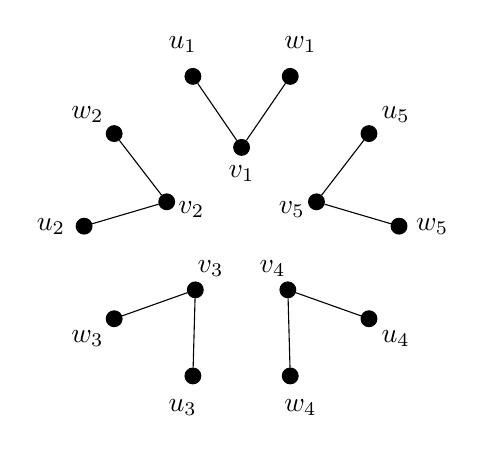
\begin{tikzpicture}

\def \iN {5}
\def \oN {10}
{
 \foreach \s in {1,...,\iN}
 {
  \node[vertex] (i\s) at ({90+360/\iN * (\s - 1)}:1cm){};% {$\s$};
  \node at ({90+360/\iN * (\s - 1)}:0.67cm){$v_\s$};
  \node at ({90+360/\iN * (\s - 0.75)}:2.42cm){$u_\s$};
  \node at ({90+360/\iN * (\s - 1.25)}:2.42cm){$w_\s$};
 }
 \foreach \s in {1,...,\oN}
 {
  \node[vertex] (o\s) at ({360/\oN * (\s - 1)}:2cm){};% {$\s$};
 }
}

\ifthenelse{\equal{\j}{1}}{
\path
(i1) edge (i2)
(i2) edge (i3)
(i3) edge (i4)
(i4) edge (i5)
(i5) edge (i1)
(o2) edge (o3)
(o4) edge (o5)
(o6) edge (o7)
(o8) edge (o9)
(o10) edge (o1);
\node[font=\Huge] at (3.8cm,0) {$\rightsquigarrow$};
}
{
\path
(i1) edge (o3) edge (o4)
(i2) edge (o5) edge (o6)
(i3) edge (o7) edge (o8)
(i4) edge (o9) edge (o10)
(i5) edge (o1) edge (o2);
}
\end{tikzpicture}
\hspace{0.5cm}
}
\end{center}

\caption{\label{fig:cycle-switching}A switching with $\ell=5$ (unaffected
edges and vertices are not pictured).}


\end{figure}


The typical application of a switching is to estimate the relative
sizes of some subsets of $\Om$, by analysing the ``flow'' of switchings
between the subsets. The switching is generally designed in such a
way that this ``flow'' is maximized in a certain ``direction''.
See \cite{HM10} for a discussion of switchings in generality.

For our case, define $S\left(k\right)$ to be the set of $d$-regular
graphs with exactly $k$ cycles of length $\ell$. The switching in
\ref{def:cycle-switching} has been chosen so that it attempts to
remove exactly one short cycle in a graph, so that for each $k$ the
``flow'' between $S\left(k\right)$ and $S\left(k-1\right)$ is
large.

In \cite[Section 3]{MWW04}, an estimate was obtained for the average
number of ways $F\left(k\right)$ to ``switch into $S\left(k-1\right)$''
from $S\left(k\right)$ (that is, the average number of $G'\in S\left(k-1\right)$
satisfying $G\rightsquigarrow G'$, where $G$ ranges over $S\left(k\right)$).
Similarly, an estimate was obtained for the average number of ways
$B\left(k-1\right)$ to ``switch from $S\left(k\right)$'' into
$S\left(k-1\right)$ (that is, the average number of $G\in S\left(k\right)$
satisfying $G\rightsquigarrow G'$, where $G'$ ranges over $S\left(k-1\right)$).
Then, $S\left(k\right)F\left(k\right)=S\left(k-1\right)B\left(k-1\right)$
is the number of pairs $\left(G,G'\right)\in S\left(k\right)\times S\left(k-1\right)$
with $G\rightsquigarrow G'$.

The estimates on $F\left(k\right)$ and $B\left(k\right)$ can be
combined for an estimate of 
\begin{equation}
\frac{\Pr\left(\X_{\ell,n}^{\left(d\right)}=k\right)}{\Pr\left(\X_{\ell,n}^{\left(d\right)}=0\right)}=\frac{S\left(k\right)}{S\left(0\right)}=\frac{B\left(0\right)\dots B\left(k-1\right)}{F\left(1\right)\dots F\left(k\right)},\label{eq:switching-quotient}
\end{equation}
which can then be used to estimate the distribution of $\X_{\ell,n}^{\left(d\right)}$.


\subsubsection{Stein's Method and Switchings}

\global\long\def\fG{\mathfrak{G}}


Obvious parallels can be drawn between the application of switchings
in \cite{MWW04} and the application of Stein's method in \ref{example:poisson-connecting-operator}.
$F\left(k\right)$ can be interpreted as the ``probability'' that
the (``forwards'') switching ``destroys a cycle'', and $B\left(k\right)$
can be interpreted as the ``probability'' that the ``backwards''
switching ``creates a cycle'', both given that there are $k$ existing
cycles. These are analogous to the probabilities $\Pr\left(\X_{2}=\X_{1}-1|\X_{1}\right)$
and $\Pr\left(\X_{2}=\X_{1}+1|\X_{1}\right)$ that must be estimated
in \ref{example:poisson-connecting-operator}.

The idea, then, is to use a switching to define a suitable exchangeable
pair, and to adapt the switching estimates for use with Stein's method.
There are two main advantages of this approach over a bare-hands switching
argument. First, a regular switching argument requires individual
estimates of each $F\left(k\right)$ and $B\left(k\right)$, but Stein's
method allows us to estimate the relevant probabilities only in expectation
(effectively, we are only estimating $\E\left[\lambda-cB\left(\X\right)\right]$
and $\E\left[\X-cF\left(\X\right)\right]$, where $\lambda$ is the
parameter of the approximating Poisson). Second, our final estimate
is likely to be sharper when using Stein's method, because we can
take advantage of the sophisticated estimates developed for Stein's
method rather than using elementary ad-hoc estimates.

The idea is that a switching $\rightsquigarrow$ defines a graph $\fG$
with an edge for every pair $\left(G,G'\right)$ with $G\rightsquigarrow G'$,
whose edges we can weight if desired. Loops are then added as necessary
to so that each vertex has the same weight $\Delta$. By \ref{prop:graph-to-markov},
$\fG$ induces a reversible Markov \textbf{c}hain with uniform stationary
distribution (in our case $\rG nd)$, which corresponds to an exchangeable
pair $\mathbf{G}=\left(G_{1},G_{2}\right)$ with margins $\rG nd$.
With \ref{rem:underlying-pair}, this provides us with an exchangeable
pair $\bX=\left(\X_{1},\X_{2}\right)$ with margins $\L{\X}$ with
which to apply Stein's method.

We give a very simplified sketch of the proof of \ref{thm:short-cycles-variable}.
We use the switching in \ref{def:cycle-switching}. Assign all edges
in $\fG$ a weight of 1, and let $\X=\X_{\ell,n}^{\left(d\right)}$.
Let $F_{C}\left(G\right)$ be the number of ways to switch out of
a graph $G$ by destroying an $\ell$-cycle $C\subseteq K_{n}$. Now,
there are $\falling n{\ell}/\left(2\ell\right)$ cycles in $K_{n}$,
so 
\begin{alignat*}{1}
\E\left|\X_{1}-c\Pr\left(\X_{2}=\X_{1}+1|\X_{1}\right)\right| & \le\E\left|\sum_{C\in K_{n}}\one_{C\subseteq G_{1}}-\frac{c}{\Delta}\sum_{C\in K_{n}}F_{C}\left(G_{1}\right)\right|\\
 & \le\frac{\falling n{\ell}}{2\ell}\E\left|\one_{C\subseteq G_{1}}-\frac{c}{\Delta}F_{C}\left(G_{1}\right)\right|.
\end{alignat*}
Similarly, let $B_{C}\left(G\right)$ be the number of ways to switch
into $G$ by destroying $C$. We have 
\[
\E\left|\frac{\left(d-1\right)^{\ell}}{2\ell}-c\Pr\left(\X_{2}=\X_{1}+1|\X_{1}\right)\right|\le\frac{\falling n{\ell}}{2\ell}\E\left|\frac{\left(d-1\right)^{\ell}}{\falling n{\ell}}-\frac{c}{\Delta}B_{C}\left(G_{1}\right)\right|.
\]
Now, if $C\subseteq G$, then $F_{C}\left(G\right)$ is approximately
$\falling n{\ell}\, d^{\ell}/2^{\ell}$. To see this, note that a
switching is determined by the $\ell$ vertices $\left\{ w_{\i}\right\} _{\i}$
and a neighbour $u_{\i}$ for each. For large $n$, there are about
$\falling n{\ell}$ ways to choose the $\left\{ w_{\i}\right\} _{\i}$,
and each $w_{\i}$ has $d$ neighbors (for large $n$ these are unlikely
to interfere with each other). Because each $u_{\i}$ and $w_{\i}$
can be interchanged, resulting in the same switching, we then need
to divide by $2^{\ell}$. Similarly, let $B_{C}\left(G\right)$ be
the number of ways to switch into $G$ by destroying $C$. A switching
that destroyed $C$ to create $G$ can be identified with a path $u_{\i}v_{\i}w_{\i}$
for each $v_{\i}\in C$, and there are about ${d \choose 2}^{\ell}$
ways to choose these paths. With these esimates in mind, we choose
$c=\Delta2^{\ell}/\left(\falling n{\ell}d^{\ell}\right)$, so that
both of 
\[
\E\left|\one_{C\subseteq G_{1}}-\frac{c}{\Delta}F_{C}\left(G_{1}\right)\right|,\quad\E\left|\frac{\left(d-1\right)^{\ell}}{\falling n{\ell}}-\frac{c}{\Delta}B_{C}\left(G_{1}\right)\right|
\]
are small. This will give us a bound on 
\[
\E\left|\X_{1}-c\Pr\left(\X_{2}=\X_{1}+1|\X_{1}\right)\right|+\E\left|\frac{\left(d-1\right)^{\ell}}{2\ell}-c\Pr\left(\X_{2}=\X_{1}+1|\X_{1}\right)\right|,
\]
as is required to prove that 
\[
d_{\TV}\left(\X,\Po\left(\frac{\left(d-1\right)^{\ell}}{\falling n{\ell}}\right)\right)\approx0.
\]


\begin{comment}


\subsection{Proof of \ref{thm:short-cycles-variable}}

Let $\X=\X_{\ell,n}^{\left(d\right)}$, let $\Om$ be the set of all
$d$-regular graphs on $n$ vertices, and let $\lambda=\left(d-1\right)^{\ell}/\left(2\ell\right)\ge1$.

The approach is conceptually similar to that of \ref{example:fixed-points}.
In the case of permuations, the transposition of two random indices
is a simple and effective way to perturb a permutation in an appropriate
way to apply the method of \ref{example:poisson-connecting-operator}.
However, it is not so easy to perturb a regular graph in a way that
maintains regularity. We accomplish this with the switching from \ref{def:cycle-switching}.

\global\long\def\fG{\mathfrak{G}}


We define a multigraph $\fG$ with vertex set $\Om$. Make an edge
in $\fG$ for every pair $\left(G,G'\right)$ with $G\rightsquigarrow G'$.
Let $\Delta$ be the maximum degree so far. Add enough loops to each
vertex of $\fG$ so that $\fG$ is a $\Delta$-regular multigraph.
Recalling \ref{prop:graph-to-markov}, $\fG$ induces a reversible
Markov \textbf{c}hain on $\Om$ with stationary distribution $\rG nd$,
which corresponds to an exchangeable pair $\mathbf{G}=\left(G_{1},G_{2}\right)$
with margins $\rG nd$. With \ref{rem:underlying-pair}, this provides
us with an exchangeable pair $\bX=\left(\X_{1},\X_{2}\right)$ with
margins $\Lb{\X_{\ell,n}^{\left(d\right)}}$ to apply Stein's method.

\begin{comment!}

Is it confusing for $G_{1},G_{2}$ to be random graphs, while graphs
denoted $G$ or $G'$ generally refer to a specific, non-random graph?
Maybe I should denote particular graphs with $\om$ instead or something.

\end{comment!}

For $G\in\Om$ and an $\ell$-cycle $C$, let $F_{C}\left(G\right)$
be the number of ways to switch from $G$ by destroying $C$. That
is,
\[
F_{C}\left(G\right)=\left|\left\{ G'\in\Om:\, G\rightsquigarrow G',\, C\subseteq G,\, C\nsubseteq G'\right\} \right|,
\]
so that $\sum_{C\in K_{n}}F_{C}\left(G\right)$ is the number of ways
to switch from $G$, destroying one $\ell$-cycle. Then,
\begin{alignat*}{1}
\Pr\left(\X_{2}=\X_{1}+1|\X_{1}\right) & =\E\left[\Pr\left(\X_{2}=\X_{1}+1|G_{1}\right)|\X_{1}\right]\\
 & =\E\left[\left.\frac{1}{\Delta}\sum_{C\in K_{n}}F_{C}\left(G_{1}\right)\right|\X_{1}\right].
\end{alignat*}


\begin{todo}

Conditioning on $\X_{1}$ is annoying, I'd rather condition on $G_{1}$.
I should add a remark to this effect when introducing the method in
the theory section, and make the same adjustment to the permutations
example.

\end{todo}

Next, the automorphism group of an $\ell$-cycle has size $2\ell$,
so the number of $\ell$-cycles in $K_{n}$ is $\falling n{\ell}/\left(2\ell\right)$.
It follows that
\begin{alignat*}{1}
\E\left|\X_{1}-\frac{\Delta}{\falling n{\ell}d^{\ell}}\Pr\left(\X_{2}=\X_{1}+1|\X_{1}\right)\right| & =\E\left|\sum_{C\in K_{n}}\one_{C\subseteq G_{1}}-\frac{1}{\falling n{\ell}d^{\ell}}\sum_{C\in K_{n}}F_{C}\left(G\right)\right|\\
 & \le\frac{\falling n{\ell}}{2\ell}\E\left|\one_{C\subseteq G_{1}}-\frac{F_{C}\left(G_{1}\right)}{\falling n{\ell}d^{\ell}}\right|.
\end{alignat*}
Similarly, let $B_{C}\left(G\right)$ be the number of ways to switch
into $G$ by destroying $C$. We have
\[
\E\left|\lambda-\frac{\Delta}{\falling n{\ell}d^{\ell}}\Pr\left(\X_{2}=\X_{1}+1|\X_{1}\right)\right|\le\frac{\falling n{\ell}}{2\ell}\E\left|\frac{\left(d-1\right)^{n}}{\falling n{\ell}}-\frac{B_{C}\left(G_{1}\right)}{\falling n{\ell}d^{\ell}}\right|.
\]
The majority of this section will consist of combinatorially bounding
these expectations, resulting in the following lemmas:
\begin{lem}
\label{lem:forward-switching-bound}Uniformly in $C$,
\[
\E\left|\one_{C\subseteq G_{1}}-\frac{F_{C}\left(G_{1}\right)}{\falling n{\ell}d^{\ell}}\right|=O\left(\frac{\ell\left(d-1\right)^{2\ell-1}}{n^{\ell+1}}\right).
\]

\end{lem}

\begin{lem}
\label{lem:backward-switching-bound}Uniformly in $C$,
\[
\E\left|\frac{\left(d-1\right)^{n}}{\falling n{\ell}}-\frac{B_{C}\left(G_{1}\right)}{\falling n{\ell}d^{\ell}}\right|=O\left(\frac{\ell\left(d-1\right)^{2\ell-1}}{n\falling n{\ell}}\right).
\]

\end{lem}
After proving these lemmas, we can conclude that
\begin{alignat*}{1}
d_{\TV}\left(\X,\Po\left(\lambda\right)\right) & \le\lambda^{-1/2}\left(\E\left|\lambda-\Delta\Pr\left(\X_{2}=\X_{1}+1|\X_{1}\right)\right|+\E\left|\X_{1}-\Delta\Pr\left(\X_{2}=\X_{1}+1|\X_{1}\right)\right|\right)\\
 & =O\left(\frac{\sqrt{\ell}\left(d-1\right)^{3\ell/2-1}}{n}\right).
\end{alignat*}
This concludes the proof of \ref{thm:short-cycles-variable}.

In order to prove \ref{lem:forward-switching-bound,backward-switching-bound},
we will need a few lemmas.
\begin{lem}
Uniformly in $C$ and $G$ such that $C$ does not share an edge with
another $\ell$-cycle in $G$,
\[
F_{C}\left(G\right)\ge\falling n{\ell}d^{\ell}\left(1-\frac{2\ell\gamma\left(G\right)+O\left(\ell\left(d-1\right)^{\ell}\right)}{nd}\right),
\]
where $\gamma\left(G\right)$ is the number of $\ell$-cycles in $G$.\end{lem}
\begin{proof}
adsf\end{proof}
\begin{lem}
Uniformly in $C$ and $G$,
\[
B_{C}\left(G\right)\ge\left(d\left(d-1\right)\right)^{\ell}\left(1-\frac{O\left(\ell\left(d-1\right)^{\ell-1}\right)}{n}\right)
\]
\end{lem}
\begin{proof}
adsf
\end{proof}

\begin{proof}
[Proof of \ref{lem:forward-switching-bound}]We partition $\rG nd$
into three events:
\begin{alignat*}{1}
\A_{1} & =\left\{ G\in\Om:C\nsubseteq G\right\} ,\\
\A_{2} & =\left\{ G\in\Om:C\subseteq G,\, C\mbox{ does not share an edge with another \ensuremath{\ell}-cycle in }G\right\} ,\\
\A_{3} & =\left\{ G\in\Om:C\subseteq G,\, C\mbox{ shares an edge with another \ensuremath{\ell}-cycle in }G\right\} .
\end{alignat*}
If $G\in\A_{1}$ then $C\nsubseteq G$, and no switching can destroy
$C$, so $F_{C}\left(G\right)=0$. If $G\in\A_{3}$, then a switching
that destroys $C$ also destroys some other $\ell$-cycle, which is
not allowed in the definition of $\rightsquigarrow$. So, $F_{C}\left(G\right)=0$.
Also, note that a switching that deletes $C$ is determined by the
$\ell$ oriented edges $e_{\i}$ in the definition of $\rightsquigarrow$.
There are at most $\falling n{\ell}d^{\ell}$ ways to choose these
edges (choose the $\ell$ vertices $u_{\i}$ then choose a neighbor
$w_{\i}$ for each), so $F_{C}\le\falling n{\ell}d^{\ell}$.

It follows that
\begin{alignat*}{1}
\E\left|\one_{C\subseteq G_{1}}-\frac{F_{C}\left(G_{1}\right)}{\falling n{\ell}d^{\ell}}\right| & =\E\left[\one_{A_{1}}\left|0-0\right|+\one_{\A_{2}}\left|1-\frac{F_{C}\left(G_{1}\right)}{\falling n{\ell}d^{\ell}}\right|+\one_{\A_{1}}\left(1-0\right)\right]\\
 & =\E\left[\one_{\A_{2}}\left(1-\frac{F_{C}\left(G_{1}\right)}{\falling n{\ell}d^{\ell}}\right)\right]+\Pr\left(\A_{3}\right)\\
\end{alignat*}


Note that a switching that deletes $C$ is determined by the $\ell$
oriented edges $e_{\i}$ in the definition of $\rightsquigarrow$.
There are at most $\falling n{\ell}d^{\ell}$ ways to choose these
edges (choose the $\ell$ vertices $u_{\i}$ then choose a neighbor
$w_{\i}$ for each), so $F_{C}\le\falling n{\ell}d^{\ell}$.

, so $F_{C}\left(G\right)\le\falling n{\ell}d^{\ell}$ and
\end{proof}

\begin{proof}
[Proof of \ref{lem:backward-switching-bound}]asfd
\end{proof}
\end{comment}


\section{Further Reading}

There are many aspects of Stein's method that we were unable to cover
in this thesis.

\begin{note}Possibly mention:
\begin{itemize}
\item different distributions, both standard and ad-hoc
\item different techniques, such as zero-biasing
\item Ways to construct characterizing operators other than exchangeable
pairs
\item Active research: random matrices, semicircle laws
\end{itemize}
\end{note}

\begin{comment}

I'd like to go into a number of small examples (perhaps interspersed
in the discussion of Stein's method in Part I), but I'd like to also
go through a number of ``big'' examples. I'd like these examples
to showcase
\begin{itemize}
\item different types of results: most applications give quantitative estimates.
\cite{Joh11} gives a non-quantitative distributional convergence
result that was not previously proved using other methods. There are
also results that have no connection with distribution metrics, such
as the concentration inequalities in \cite{Ros11}. In particular,
the Latin rectangle example in \cite{Ste86} is interesting in that
the final result is not probabilistic.
\item different types of distributions: definitely at least the Poisson
and normal case, perhaps also an example of a more exotic distribution
like the one in \cite{FS12} or perturbations of Poisson/normal distributions
as in \cite{BCX07}.
\item different ways to apply stein's method: definitely exchangeable pairs
and probably size-biasing. Maybe also Zero-bias coupling.
\end{itemize}
\end{comment}

\let\textbf\oldtextbf

\bibliographystyle{amsalpha.mod}
\bibliography{readings}

\end{document}
